You will need to add a couple of hardware components to your Cow Pi circuit before you can start this lab.

\subsection{Necessary Components}

Figure~\ref{fig:components-mk4b} shows the components you will need for the electronic combination lock.

\begin{figure}
    \centering
    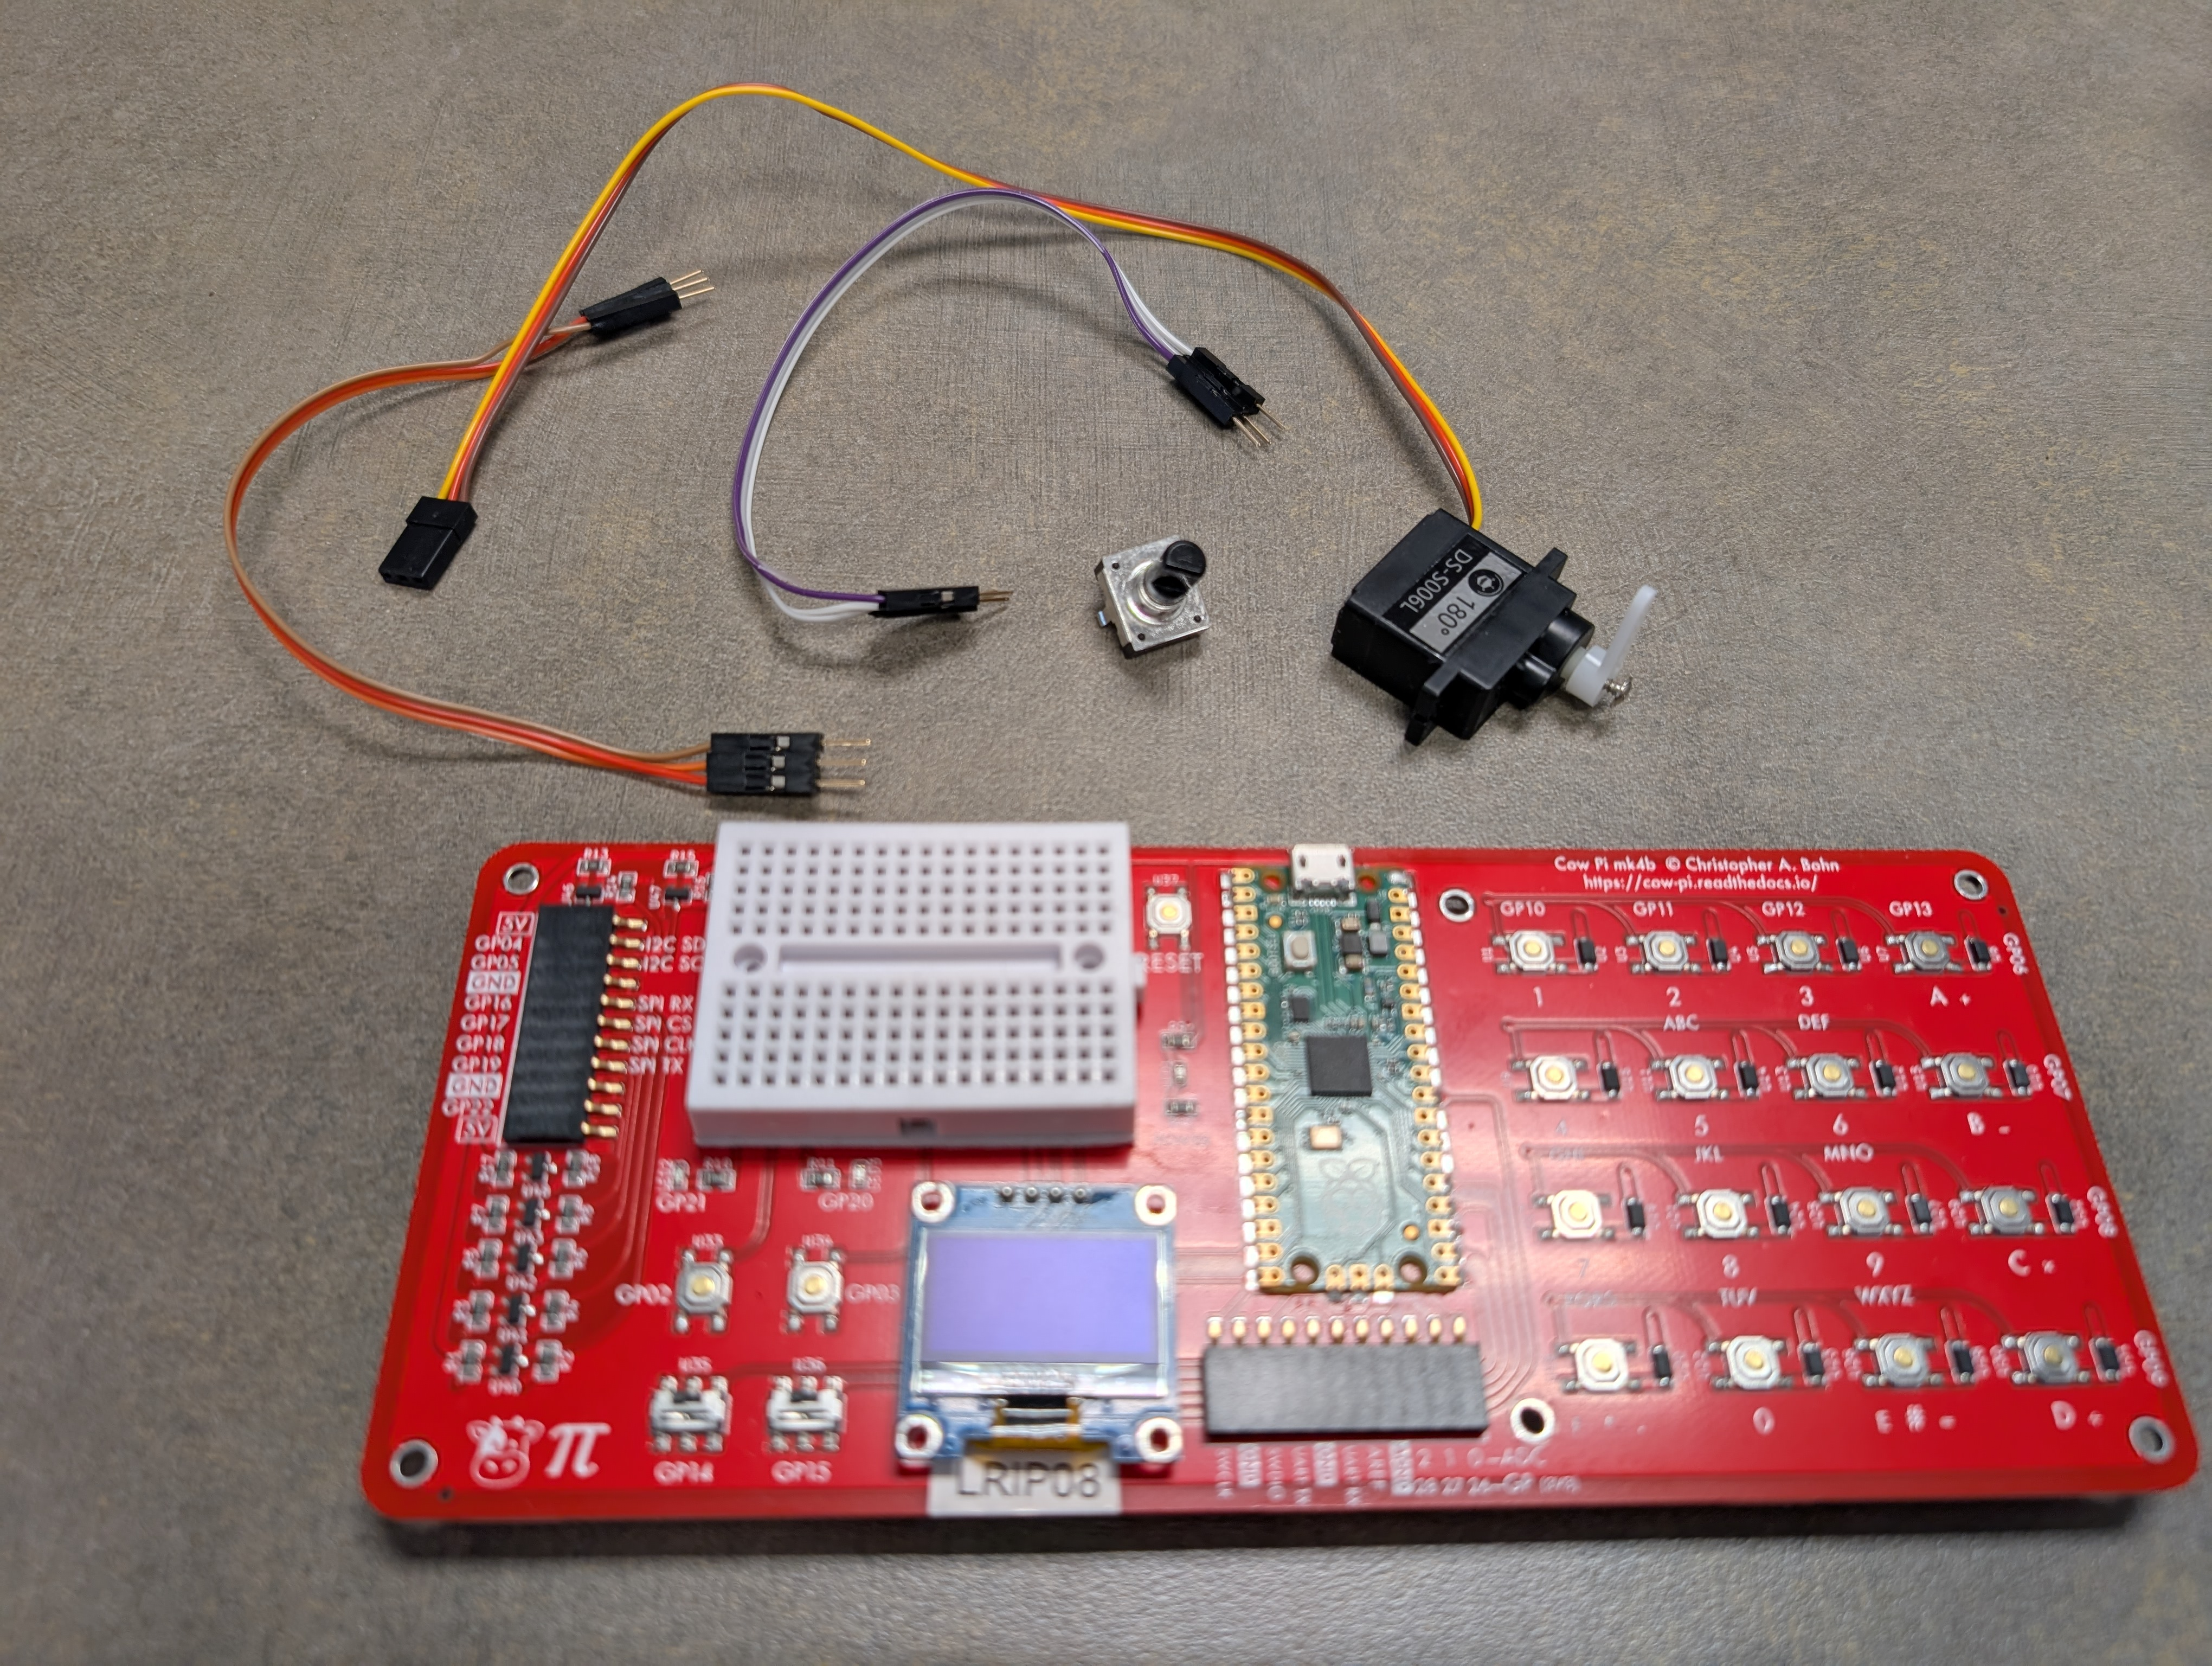
\includegraphics[width=10cm]{hardware/components}
    \caption{Components needed for the Range Finder \label{fig:components-mk4b}}
\end{figure}

You will need:
\begin{itemize}
    \item Your Cow Pi hardware circuit
    \item A rotary encoder
    \item A servomotor
    \item Six 20cm male-to-male wires
\end{itemize}

There is a labeled header on the left side of the Cow~Pi;
we will use this to connect the hardware components to the RP2040 microcontroller.

\subsection{The Mini-Breadboard on the Cow Pi}

A key feature of solderless breadboards, such as the mini-breadboard on your Cow~Pi, are the groups of 5 holes (Figure~\ref{fig:breadboard-mk4b}).
Each group of five is a \textit{terminal strip}.

\begin{figure}
    \centering
    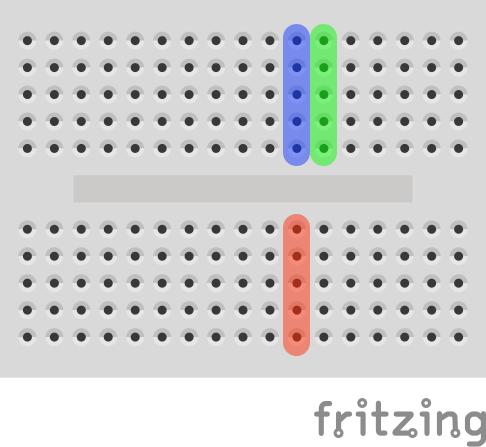
\includegraphics[height=4cm]{hardware/breadboard}
    \caption{Terminal strips on a mini-breadboard \label{fig:breadboard-mk4b}}
\end{figure}

The five holes in a terminal strip are electrically connected to each other but are electrically isolated from the other terminal strips.\footnote{
    They are isolated for DC signals, and parasitic reactance is negligible for AC signals below about 10~kHz.
}
For example, in Figure~\ref{fig:breadboard-mk4b}, all holes in the terminal strip that is highlighted in blue are connected to each other,
but they are not connected to the holes in the adjacent terminal strip highlighted in green.
Similarly, they are not connected to the holes in the red terminal strip on the other side of the gutter.

A consequence of this is that any components' connectors that are inserted into a terminal strip are connected to the connectors of other components that are inserted into the same terminal strip.

If you want to learn more, a very good overview of solderless breadboards can be found here: \url{https://learn.adafruit.com/breadboards-for-beginners?view=all}

%Figure~\ref{fig:breadboard-with-components-mk4b} shows where you will insert the hardware components for the group project.
%(The precise placement is not critical, so long as you make a note of which terminal strips you use.)
%
%\begin{figure}
%    \centering
%    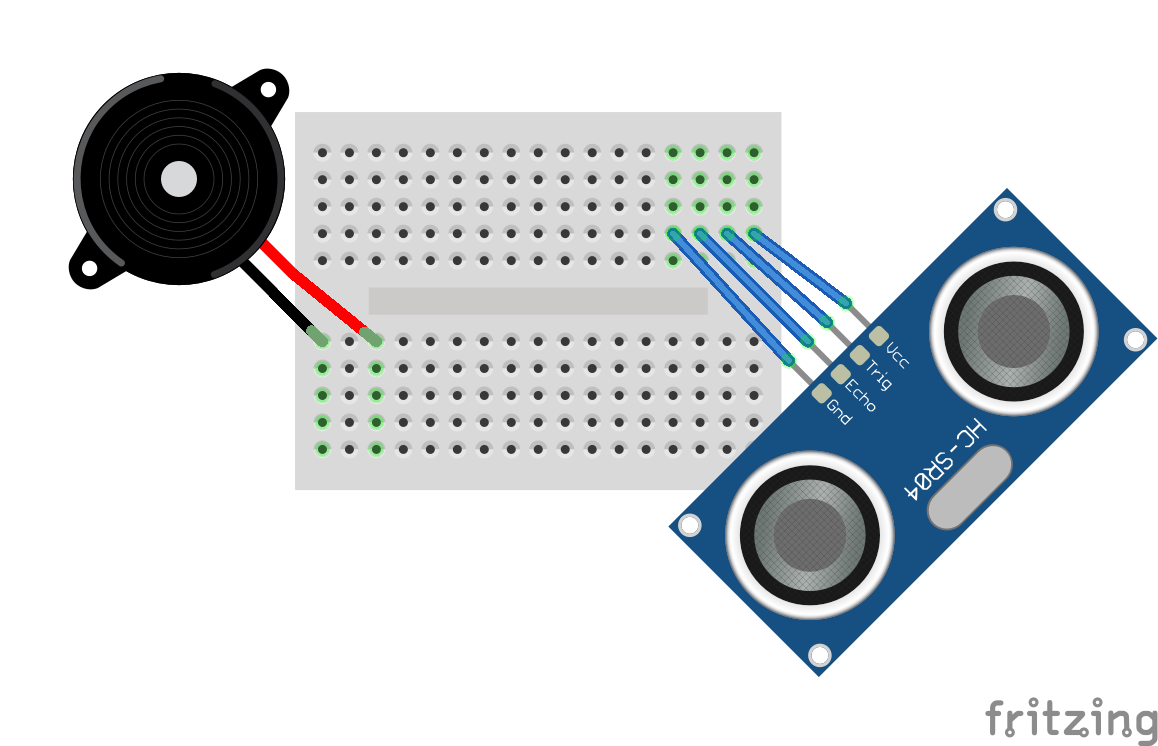
\includegraphics[height=4cm]{hardware/mk4b/breadboard-with-components}
%    \caption{Terminal strips on a mini-breadboard \label{fig:breadboard-with-components-mk4b}}
%\end{figure}


\subsection{Connecting the servomotor}

If your servomotor does not already have a servo arm attached, attach a servo arm to the motor's shaft.
See Figure~\ref{fig:servoArm}.
The orientation does not matter since we will not connect anything to the servo -- we are simply using the servomotor to simulate a lock's deadbolt mechanism,
and the arm will allow us to see the motion.
\textit{Do \underline{not} screw the arm to the motor's shaft.}
Simply let it fit snugly.


\begin{figure}
    \centering
    \subfloat[A servo arm can be attached to a servo motor.]{
        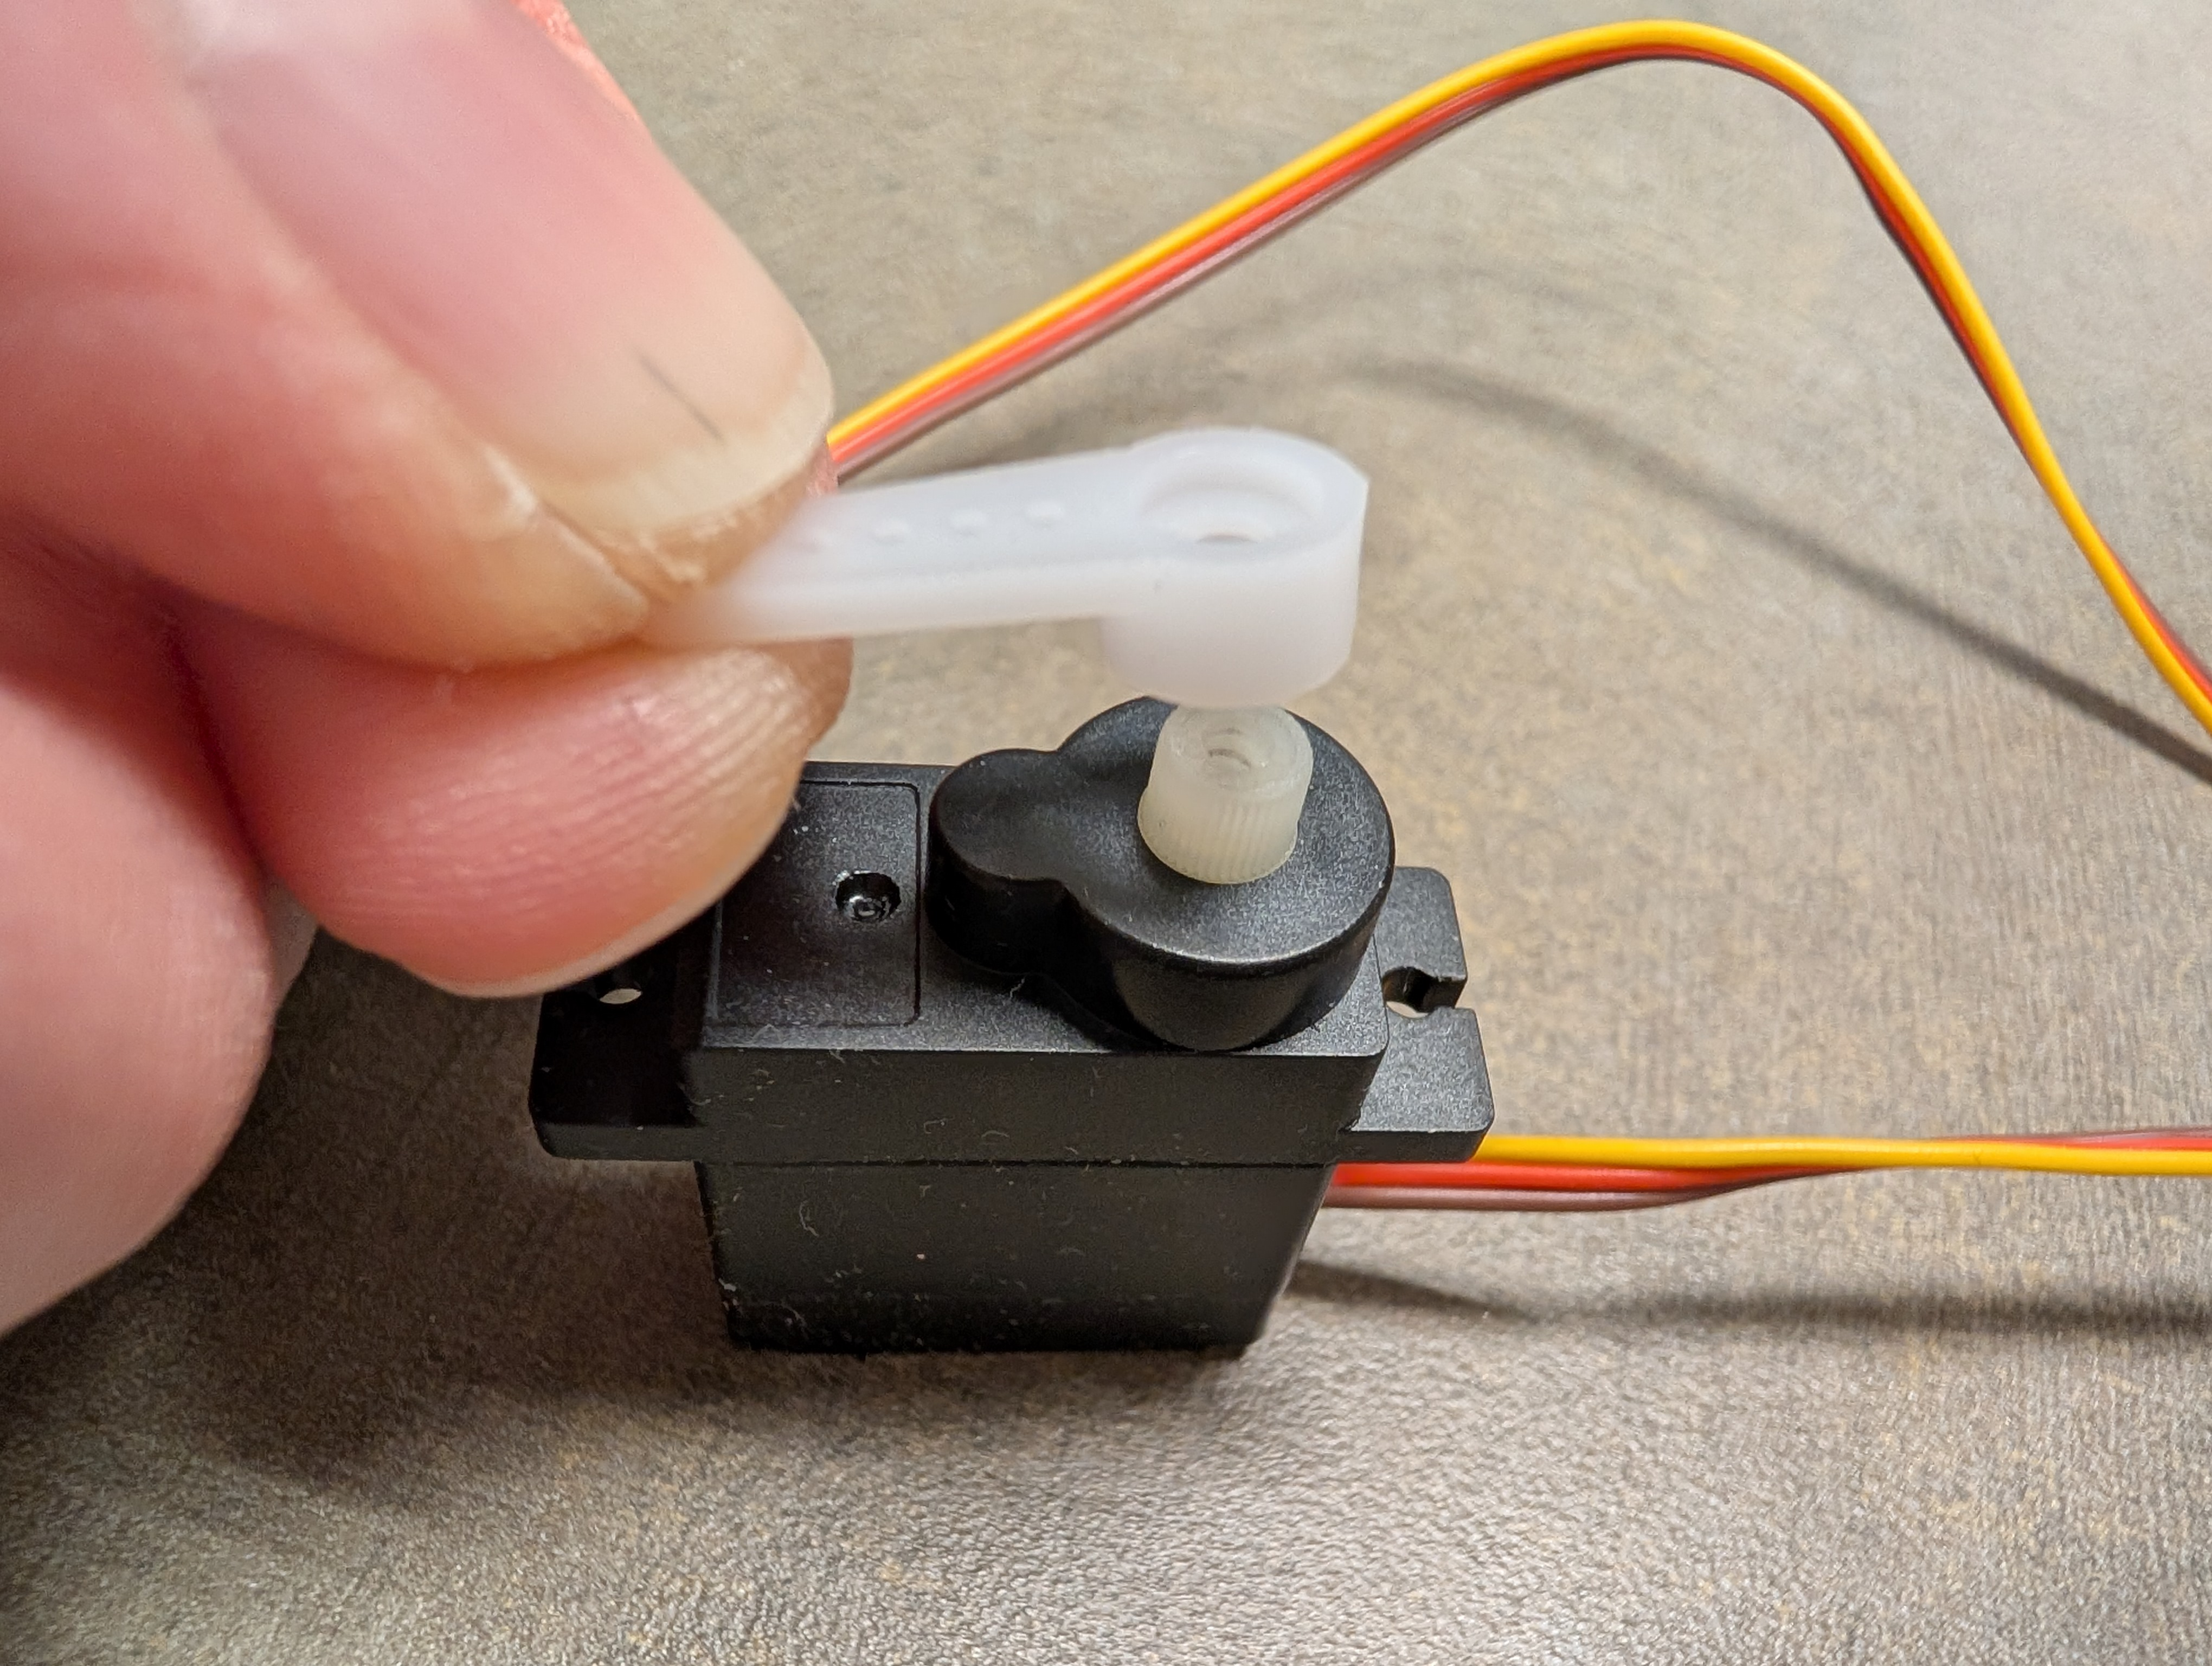
\includegraphics[height=4cm]{hardware/aboutToAttachServoArm}
%        \label{fig:attaching}
    }
    \hfil
    \subfloat[A servo arm has been attached to a servo motor.]{
        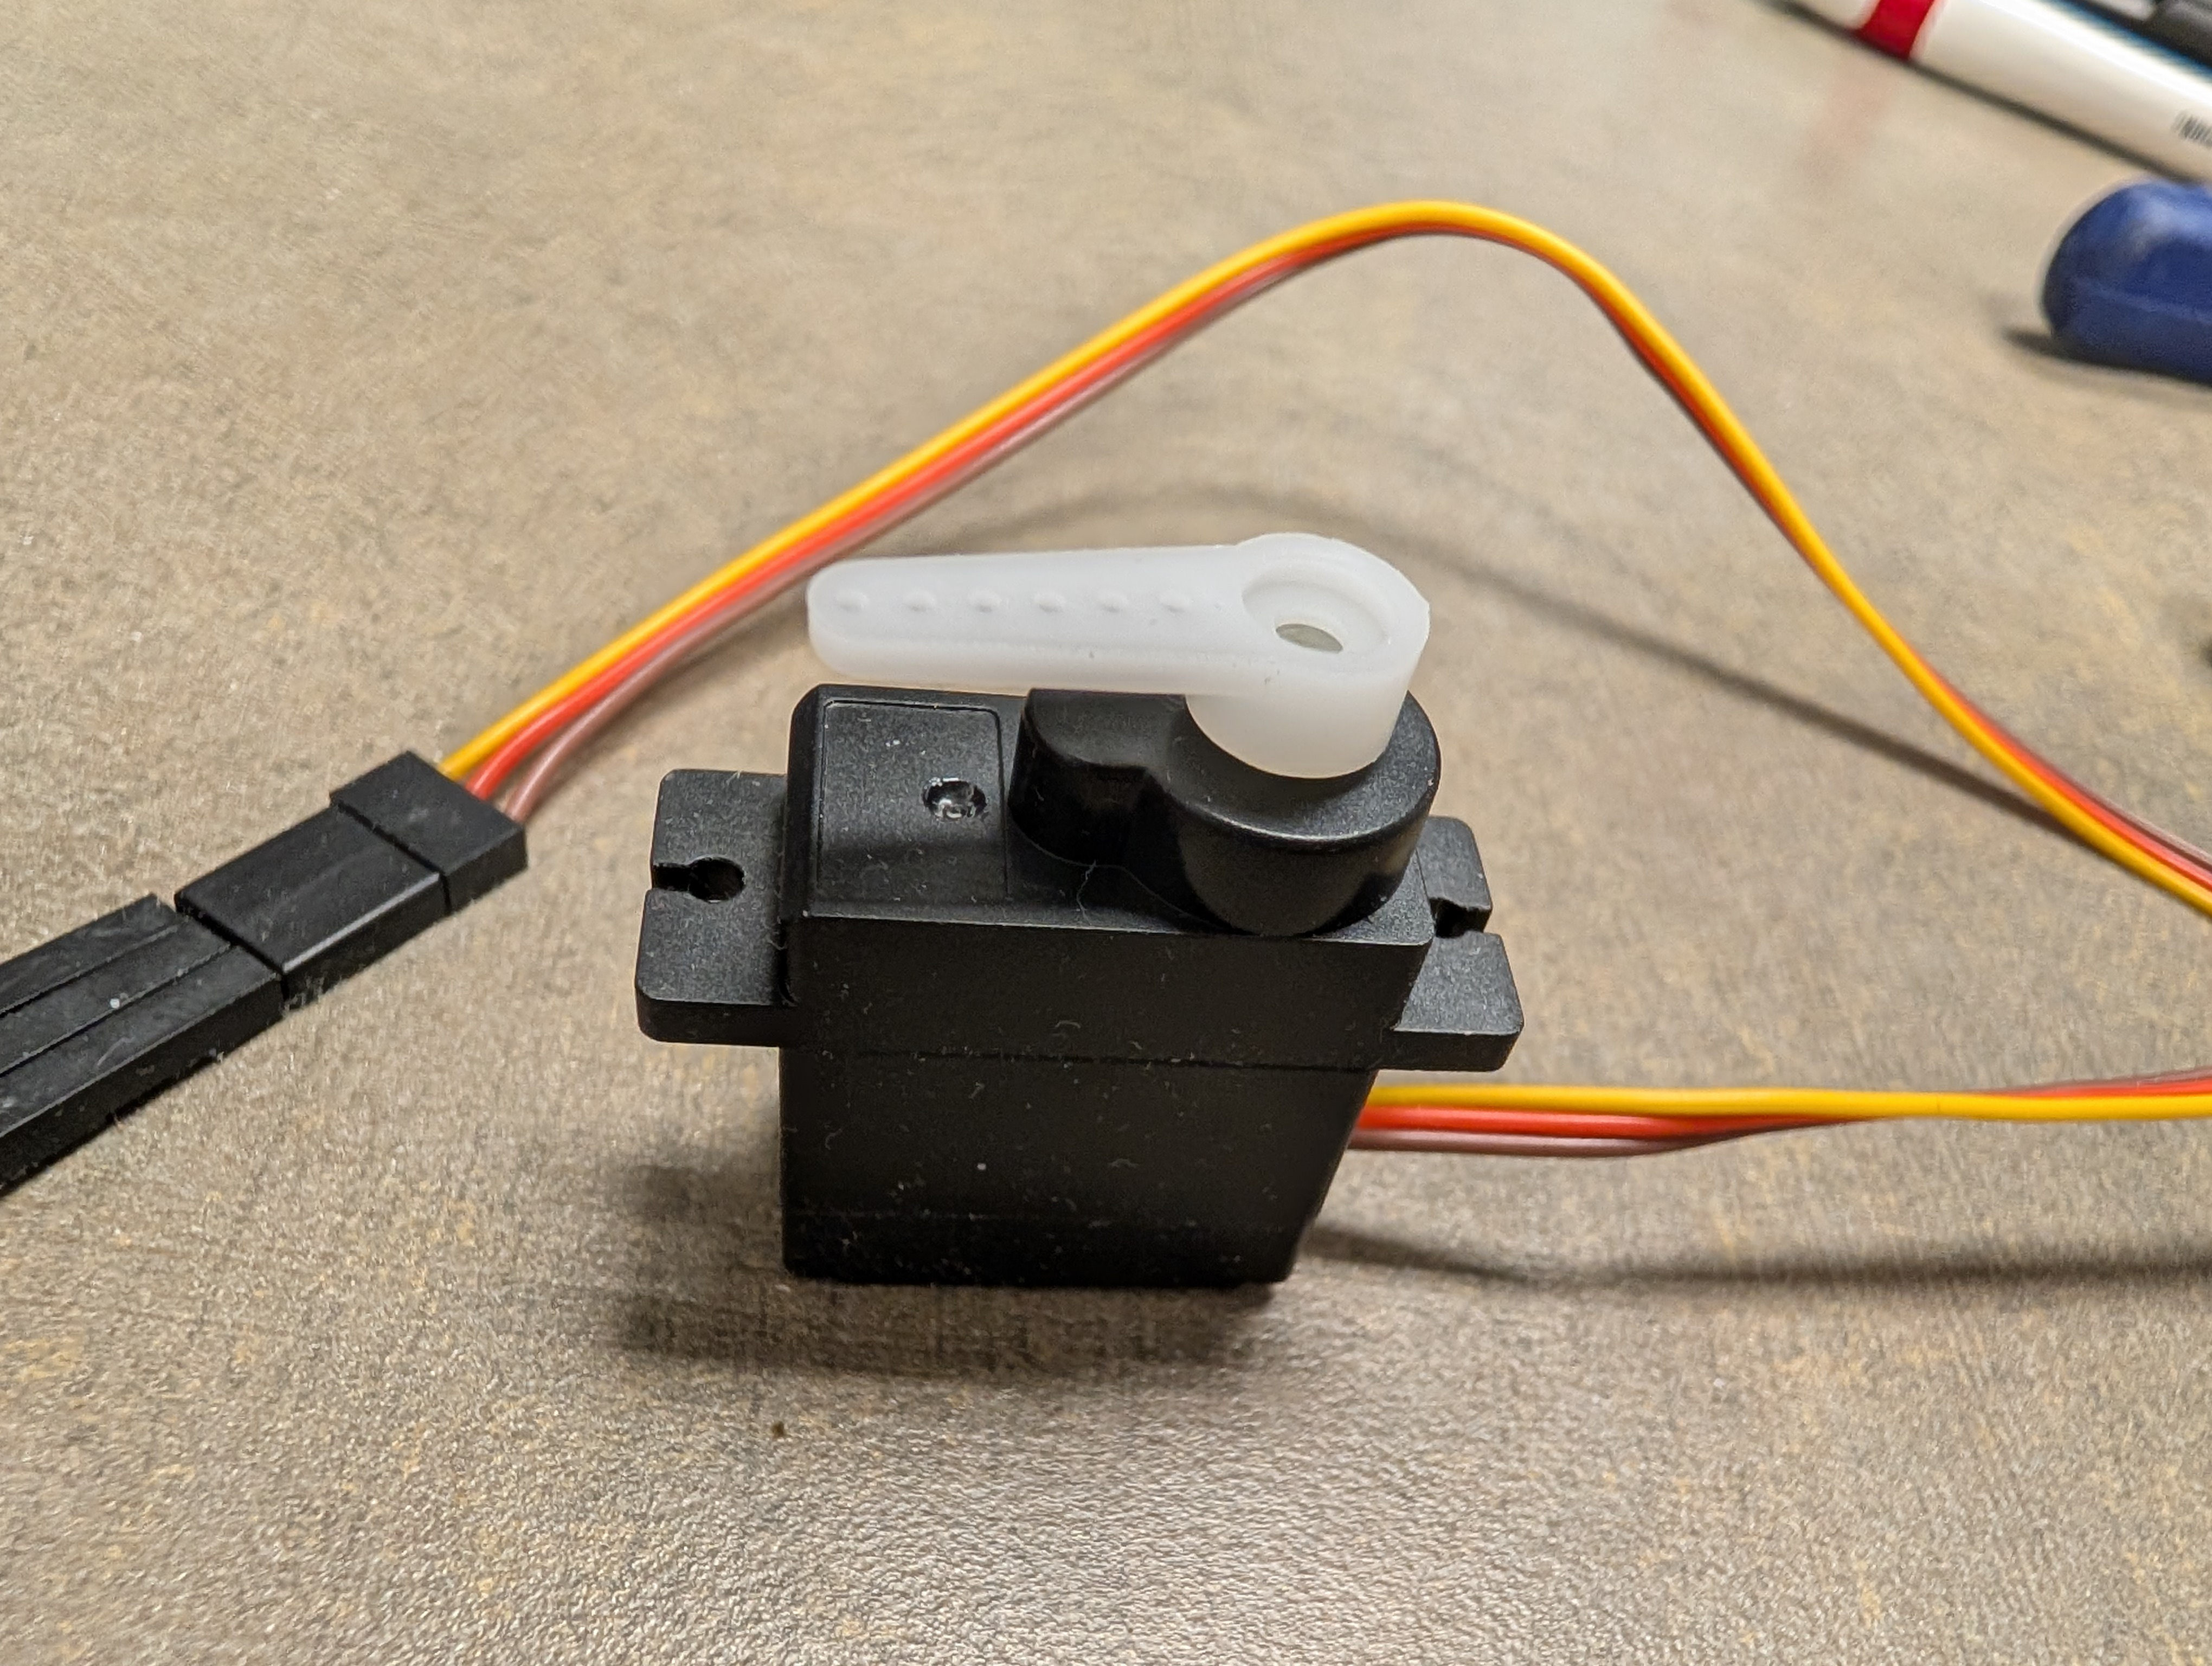
\includegraphics[height=4cm]{hardware/servoArmAttached}
%        \label{fig:attached}
    }
    \caption{Attaching a servo arm to a servo motor. \label{fig:servoArm}}
\end{figure}

\begin{description}
    \checkoffitem{Attach three to the servo's wires (Figure~\ref{fig:attachWiresToServo}).
        The colors do not need to match, but you do need to pay attention to which 20cm wire you attached to which servo wire.}
    \checkoffitem{Locate the 20cm that is attached to the servo's \textbf{red} wire. Insert the other end into a \texttt{5V} slot.}
    \checkoffitem{Locate the 20cm that is attached to the servo's \textbf{brown} wire. Insert the other end into a \texttt{GND} slot.}
    \checkoffitem{Locate the 20cm that is attached to the servo's \textbf{yelow} wire. Insert the other end into the \texttt{GP22} slot.}
    \checkoffitem{\textcolor{red}{Have someone verify that you have each wire inserted into the correct slot.}}
\end{description}


\begin{figure}
    \centering
    \subfloat[Attaching 20cm wires to servo wires.]{
        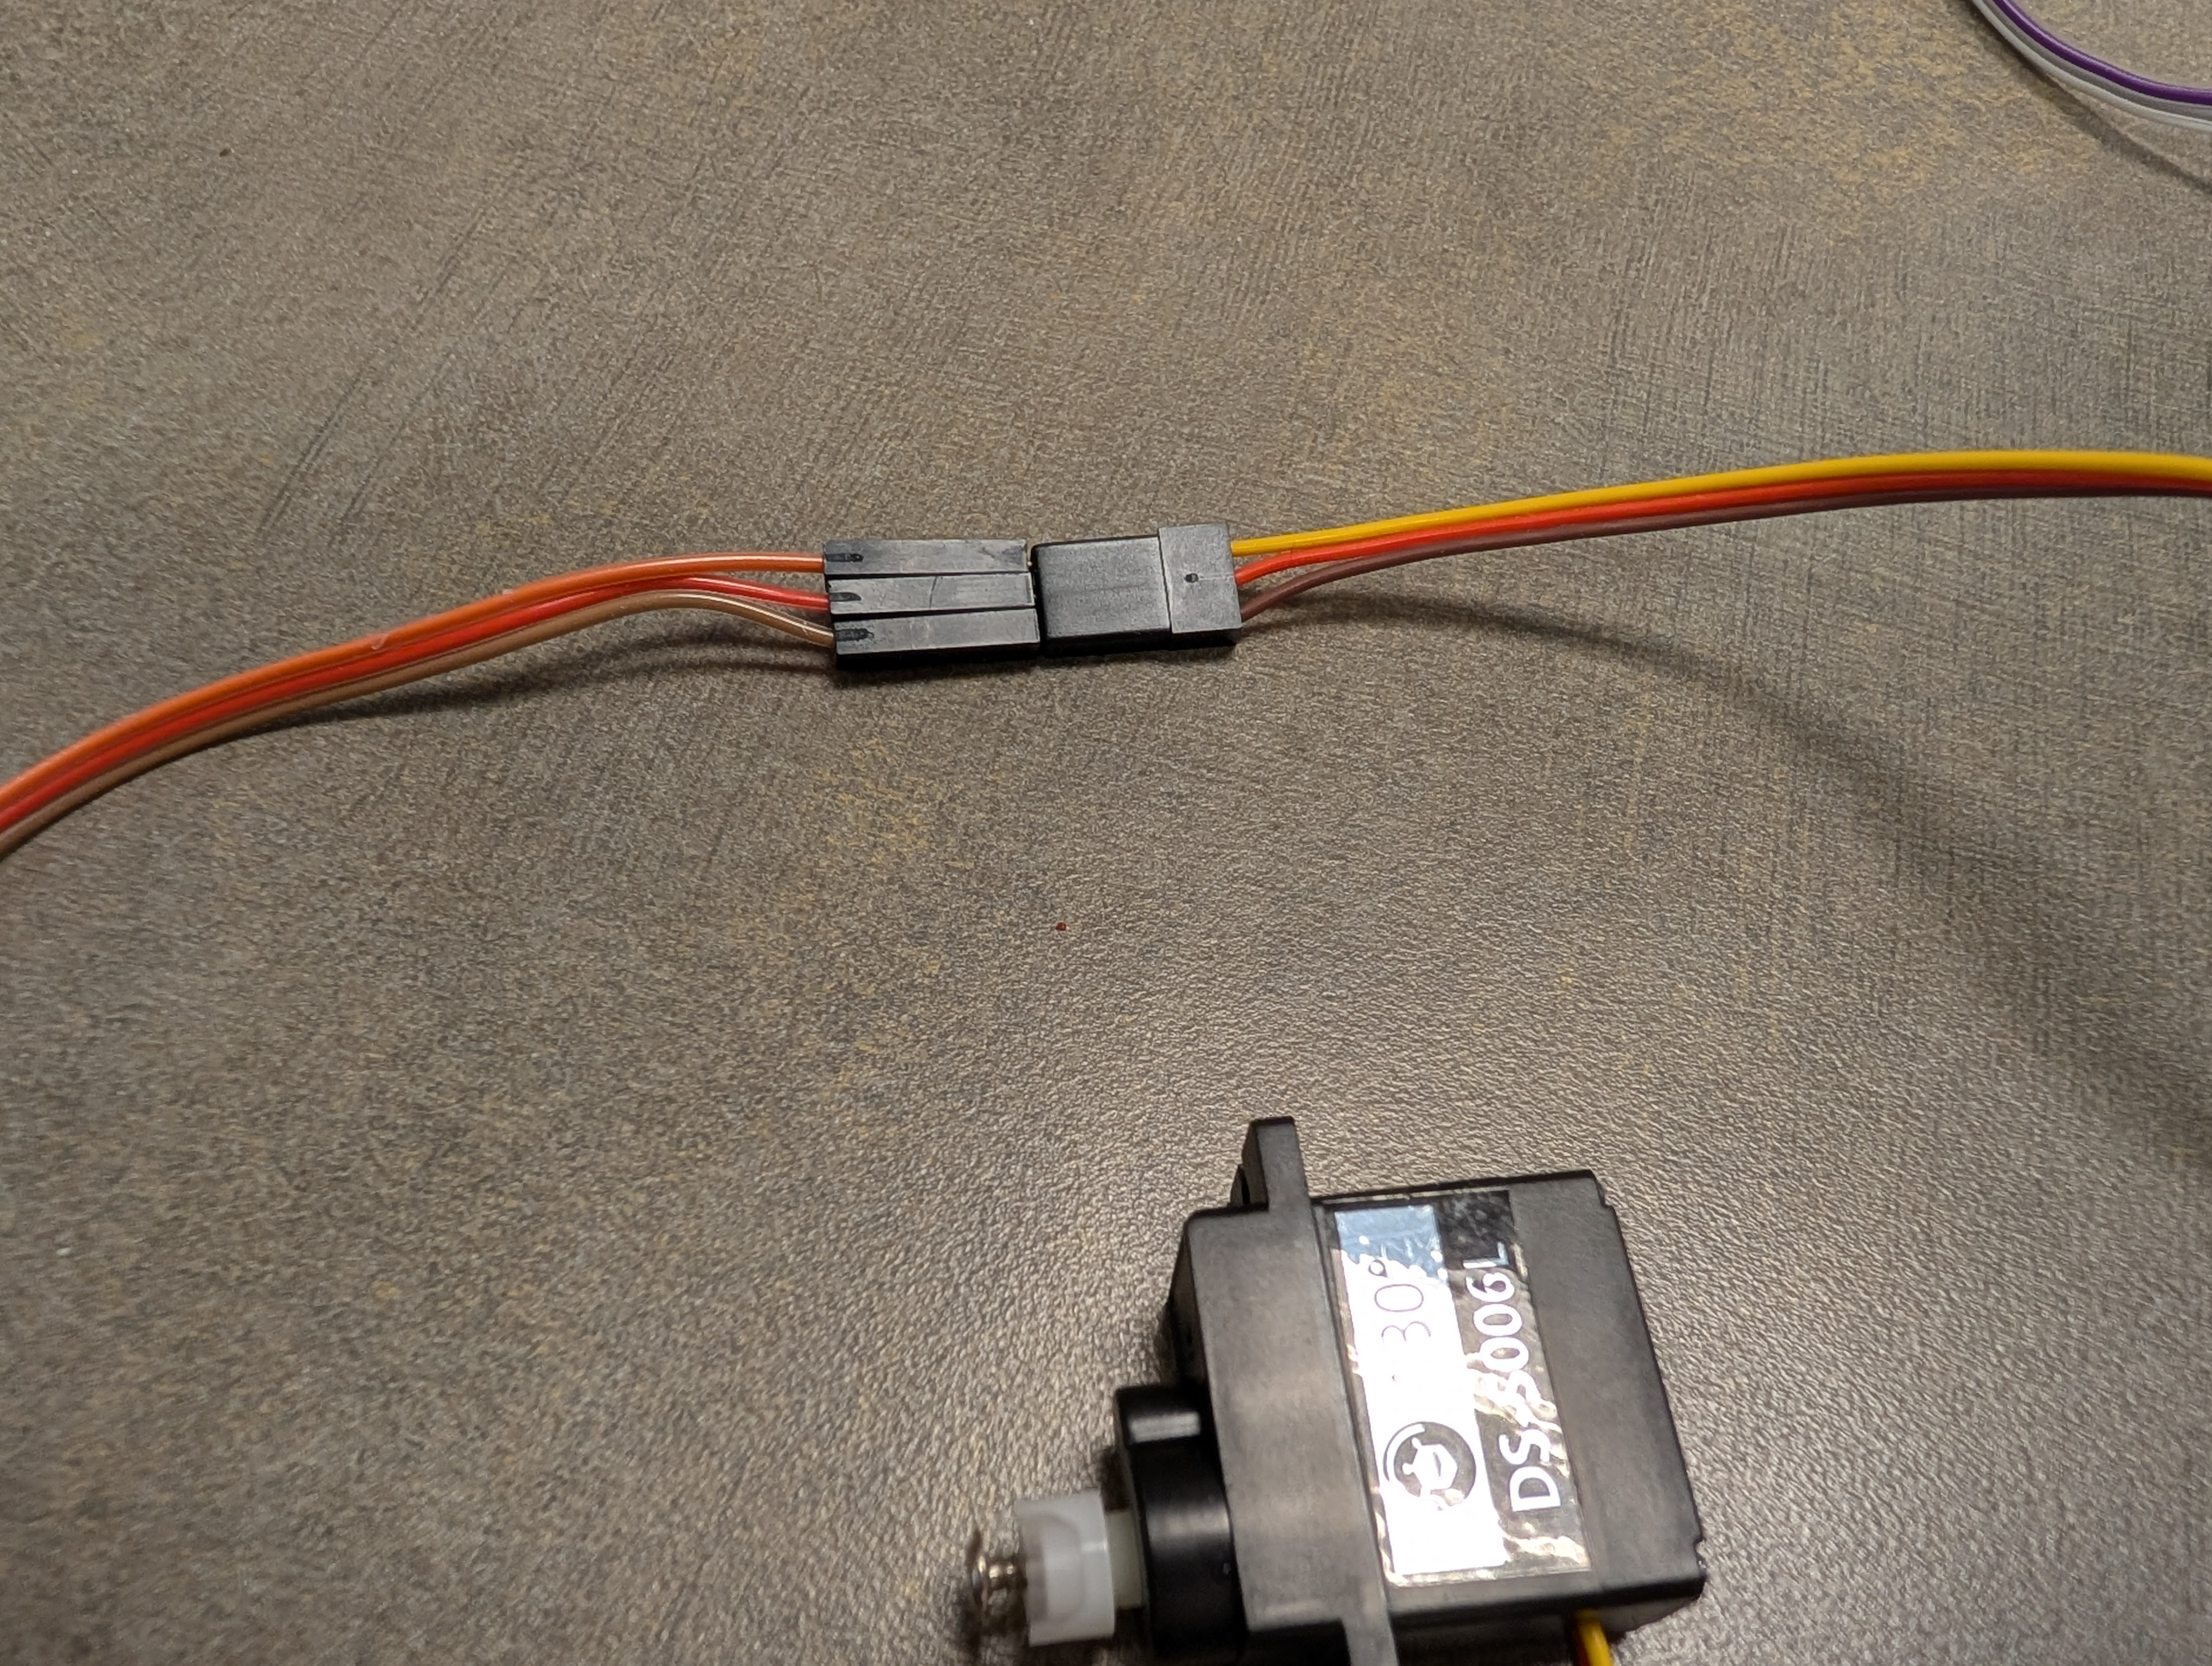
\includegraphics[height=4cm]{hardware/attachWiresToServo}
        \label{fig:attachWiresToServo}
    }
    \\
    \subfloat[Determining where to insert each wire.]{
        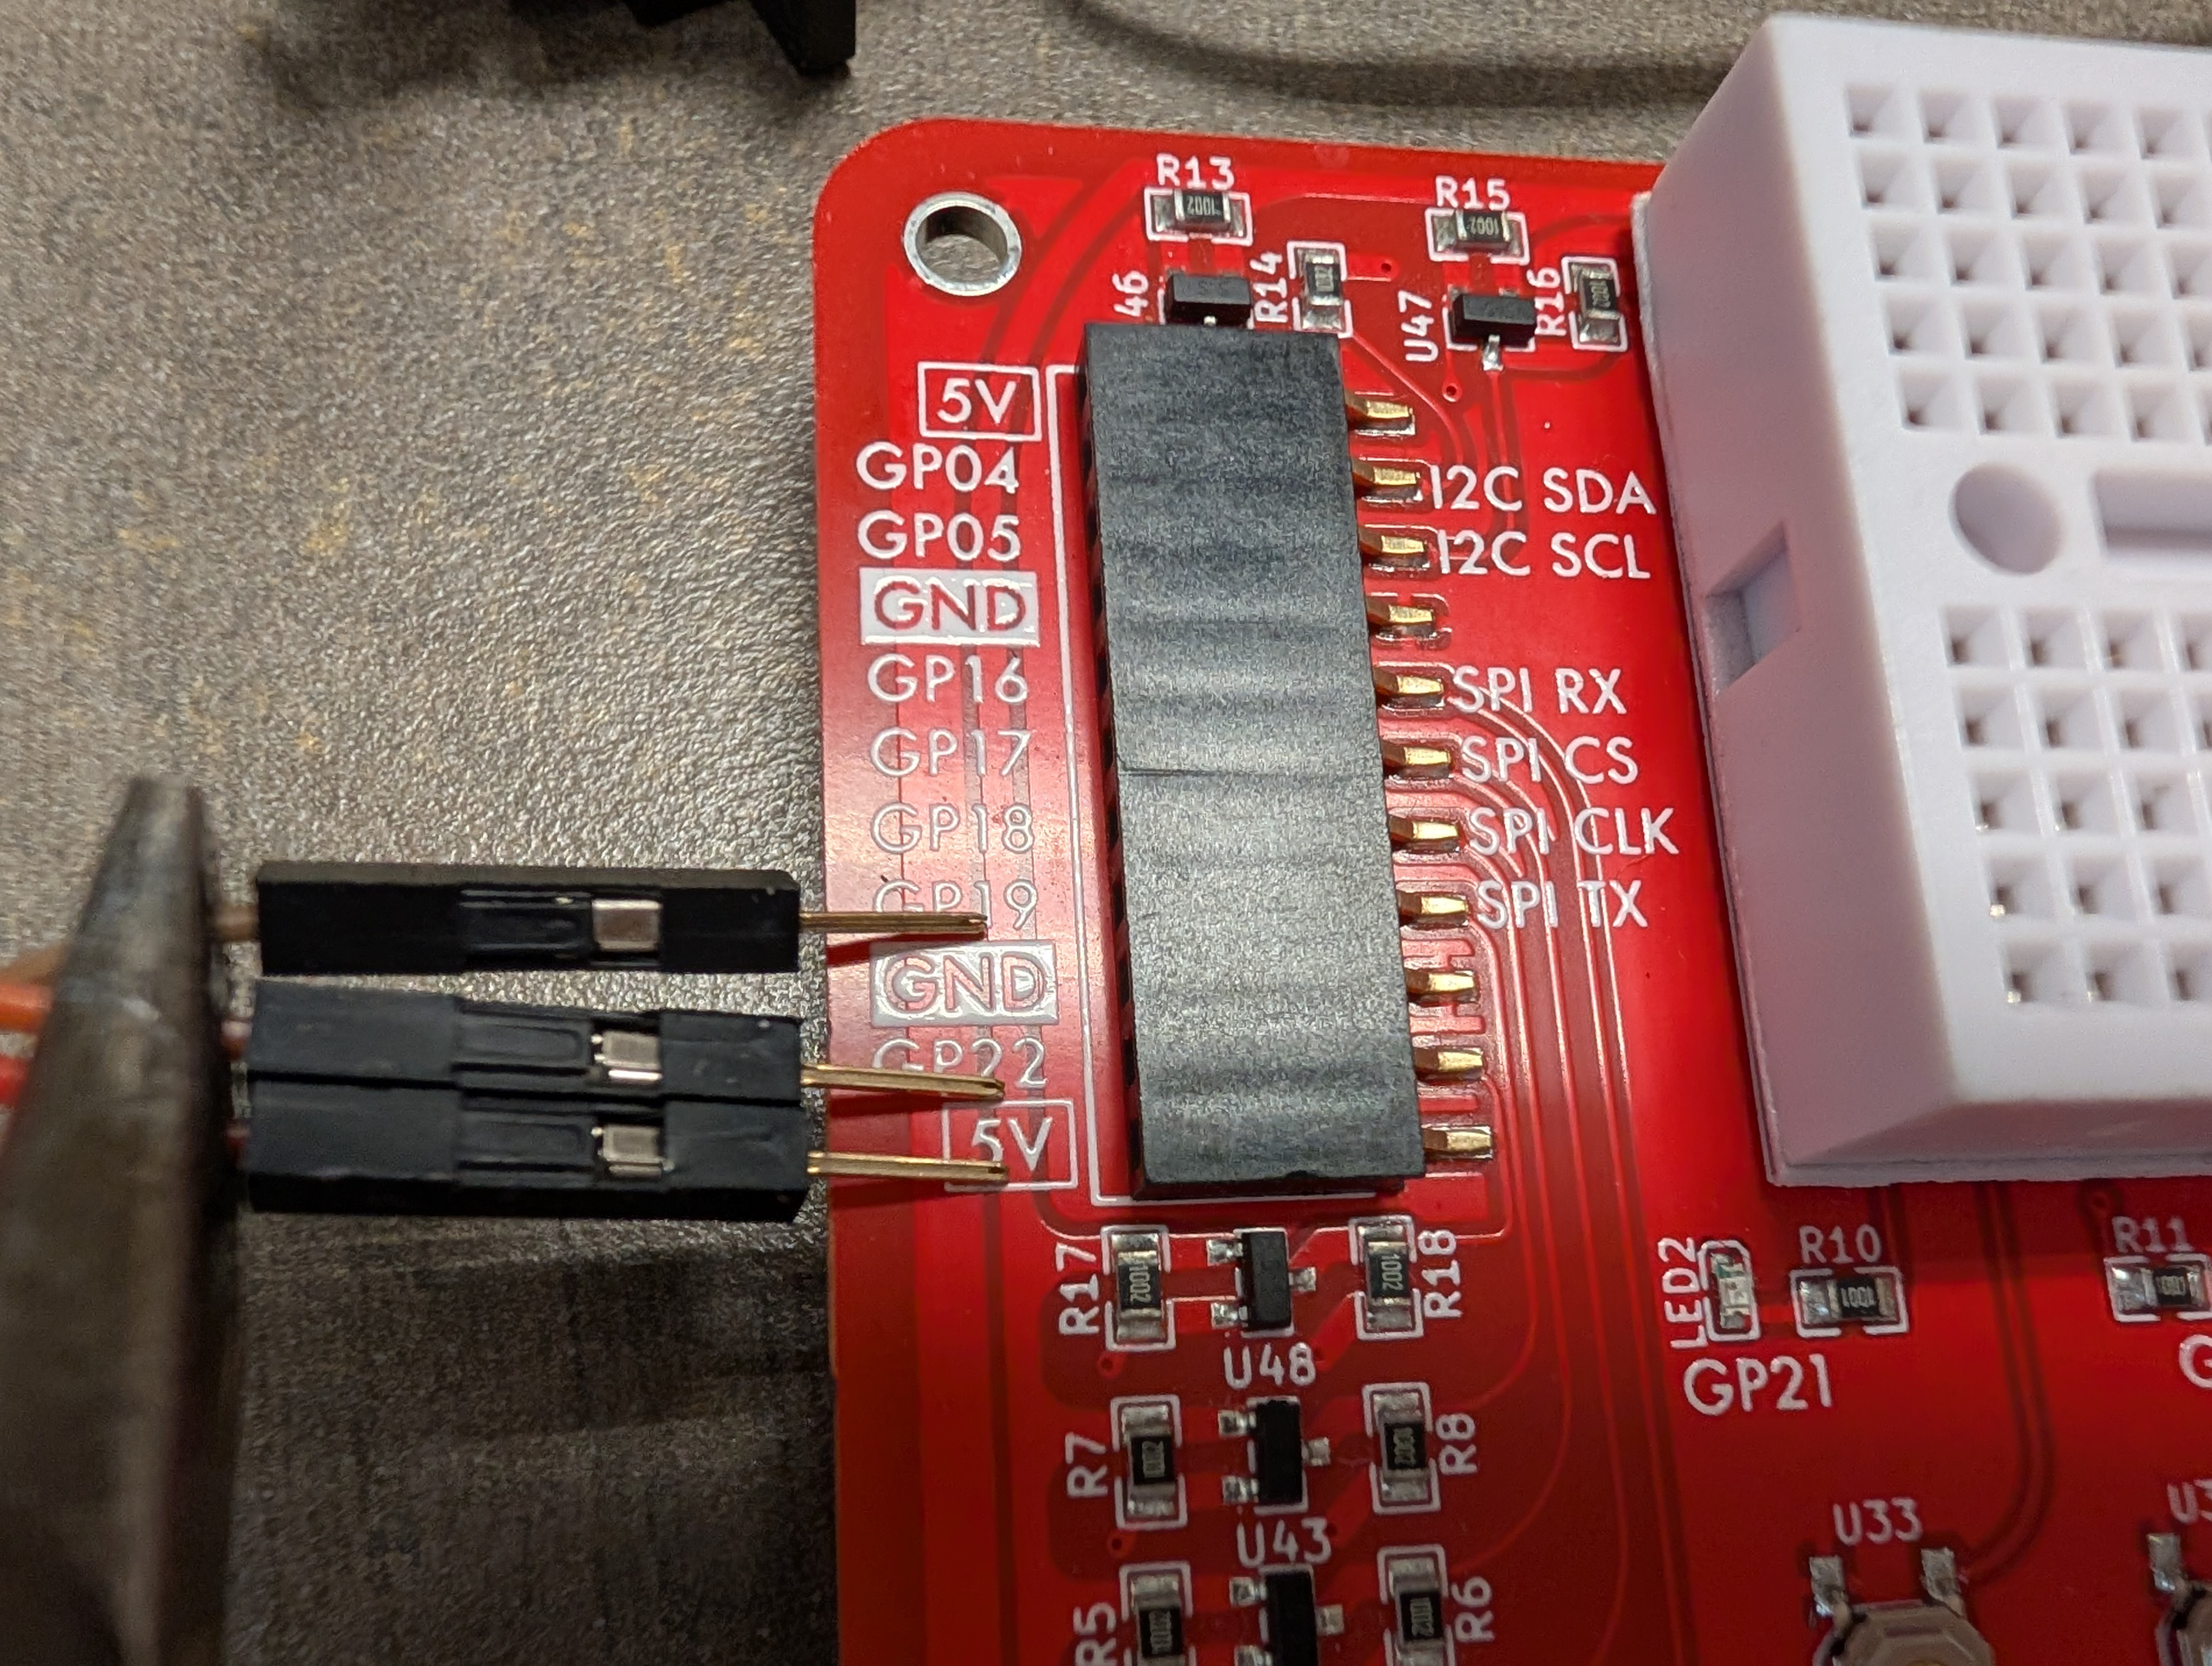
\includegraphics[height=4cm]{hardware/attachingServo}
%        \label{fig:attached}
    }
    \hfil
    \subfloat[All servo wires connected.]{
        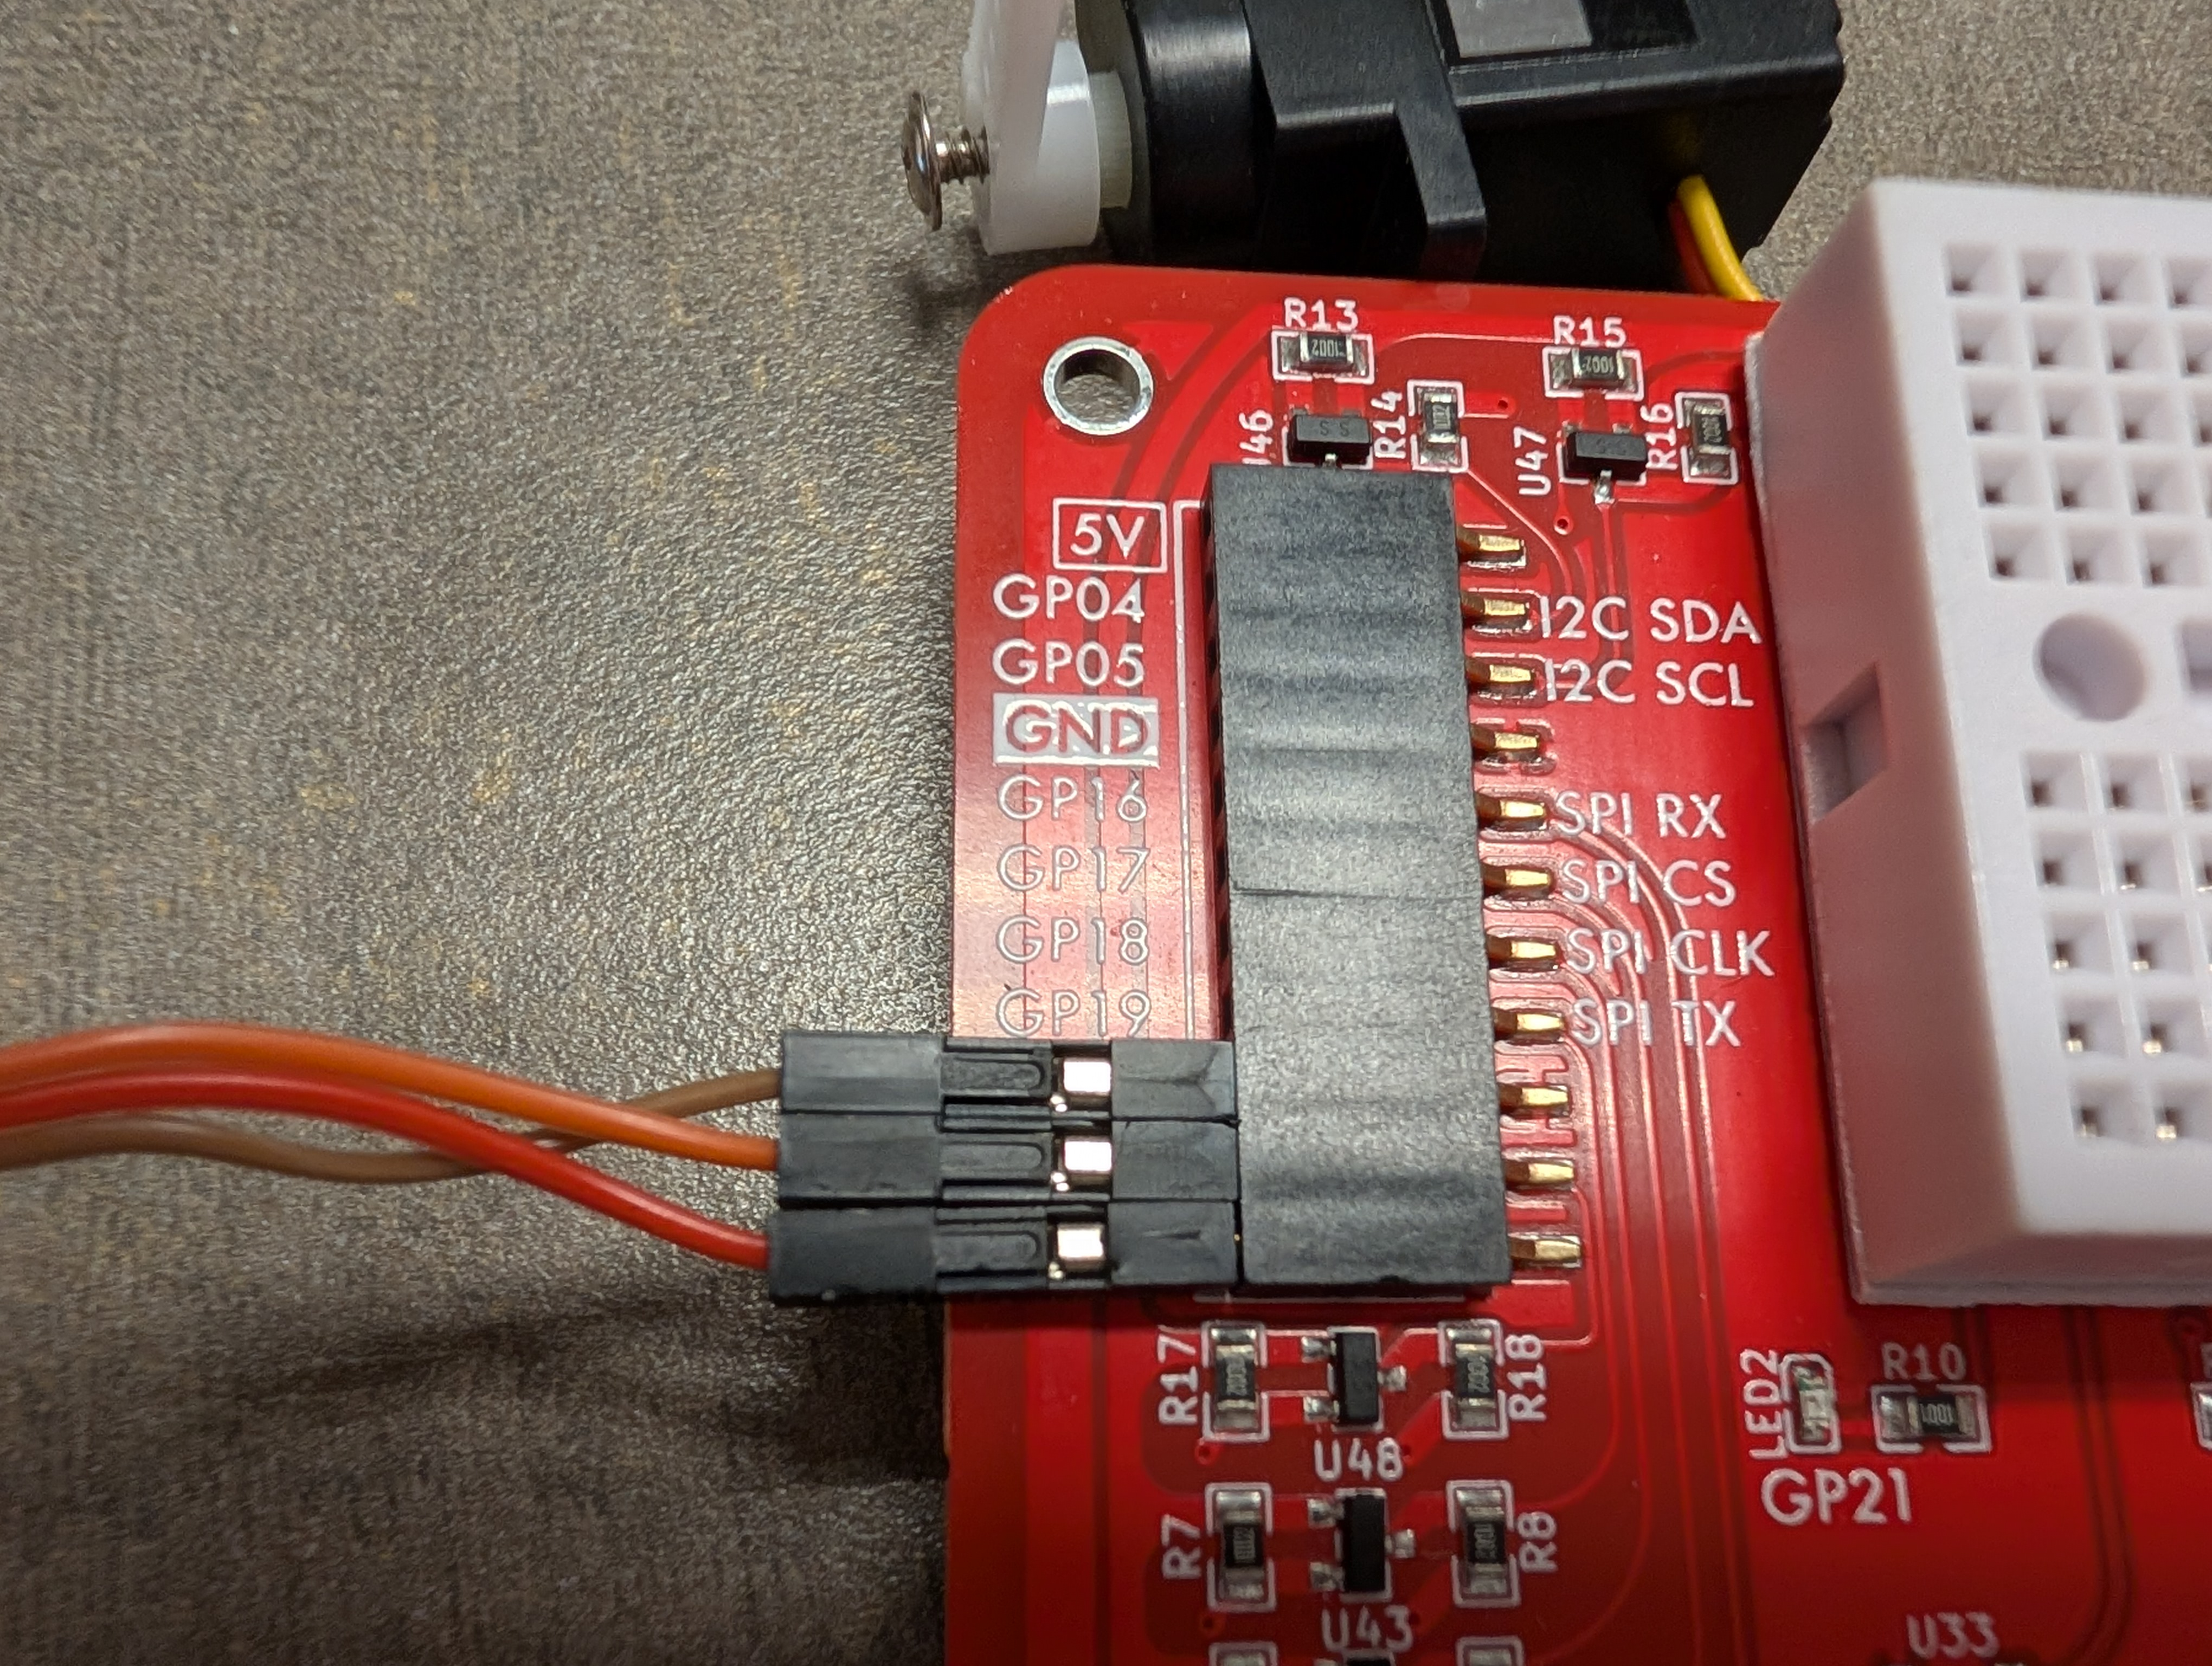
\includegraphics[height=4cm]{hardware/servoAttached}
%        \label{fig:attached}
    }
    \caption{Wiring a servo motor to the Cow~Pi. \label{fig:servoWiring}}
\end{figure}

The servo motor is now connected to the Cow~Pi's \texttt{GP22} pin.
The starter code will configure \texttt{GP22} to be an output pin.


\subsection{Connecting the Rotary Encoder}

\begin{figure}
    \centering
    \subfloat[Position the prongs into the breadboard gutter.]{
        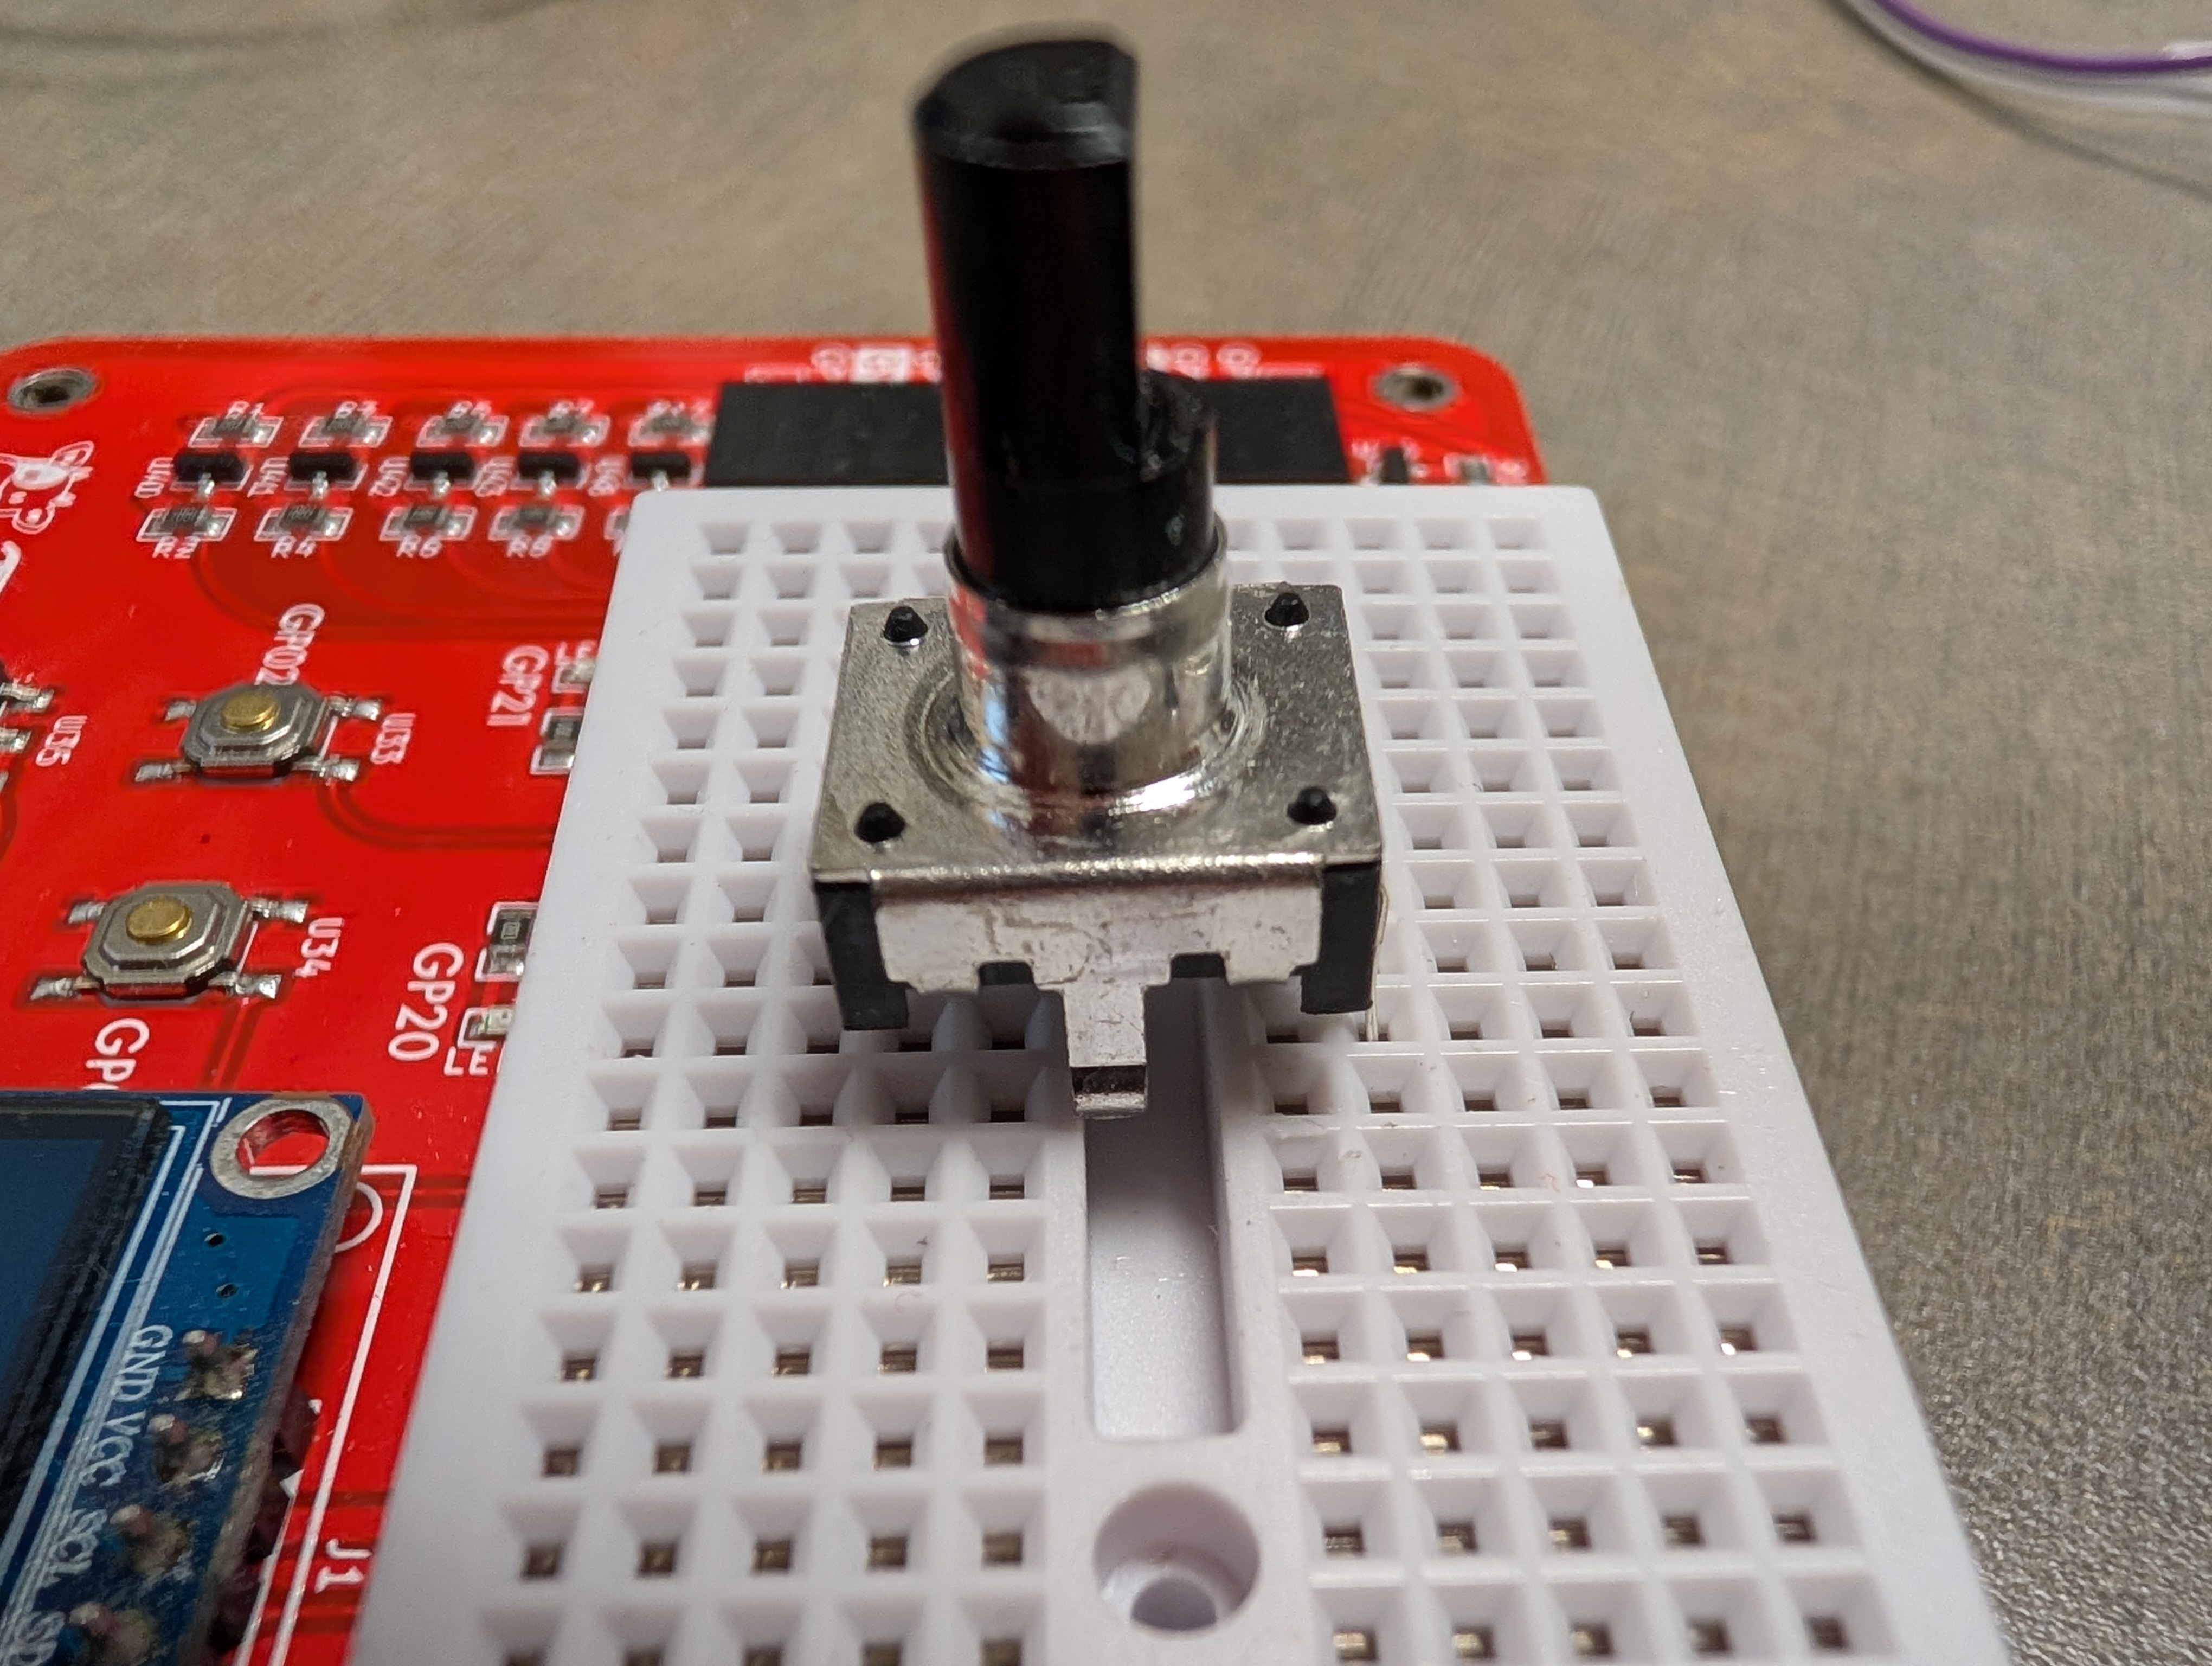
\includegraphics[height=4cm]{hardware/rotaryEncoderProngAlignment}
        \label{fig:rotaryEncoderProngs}
    }
    \hfil
    \subfloat[Placing the pins in contact point wells.]{
        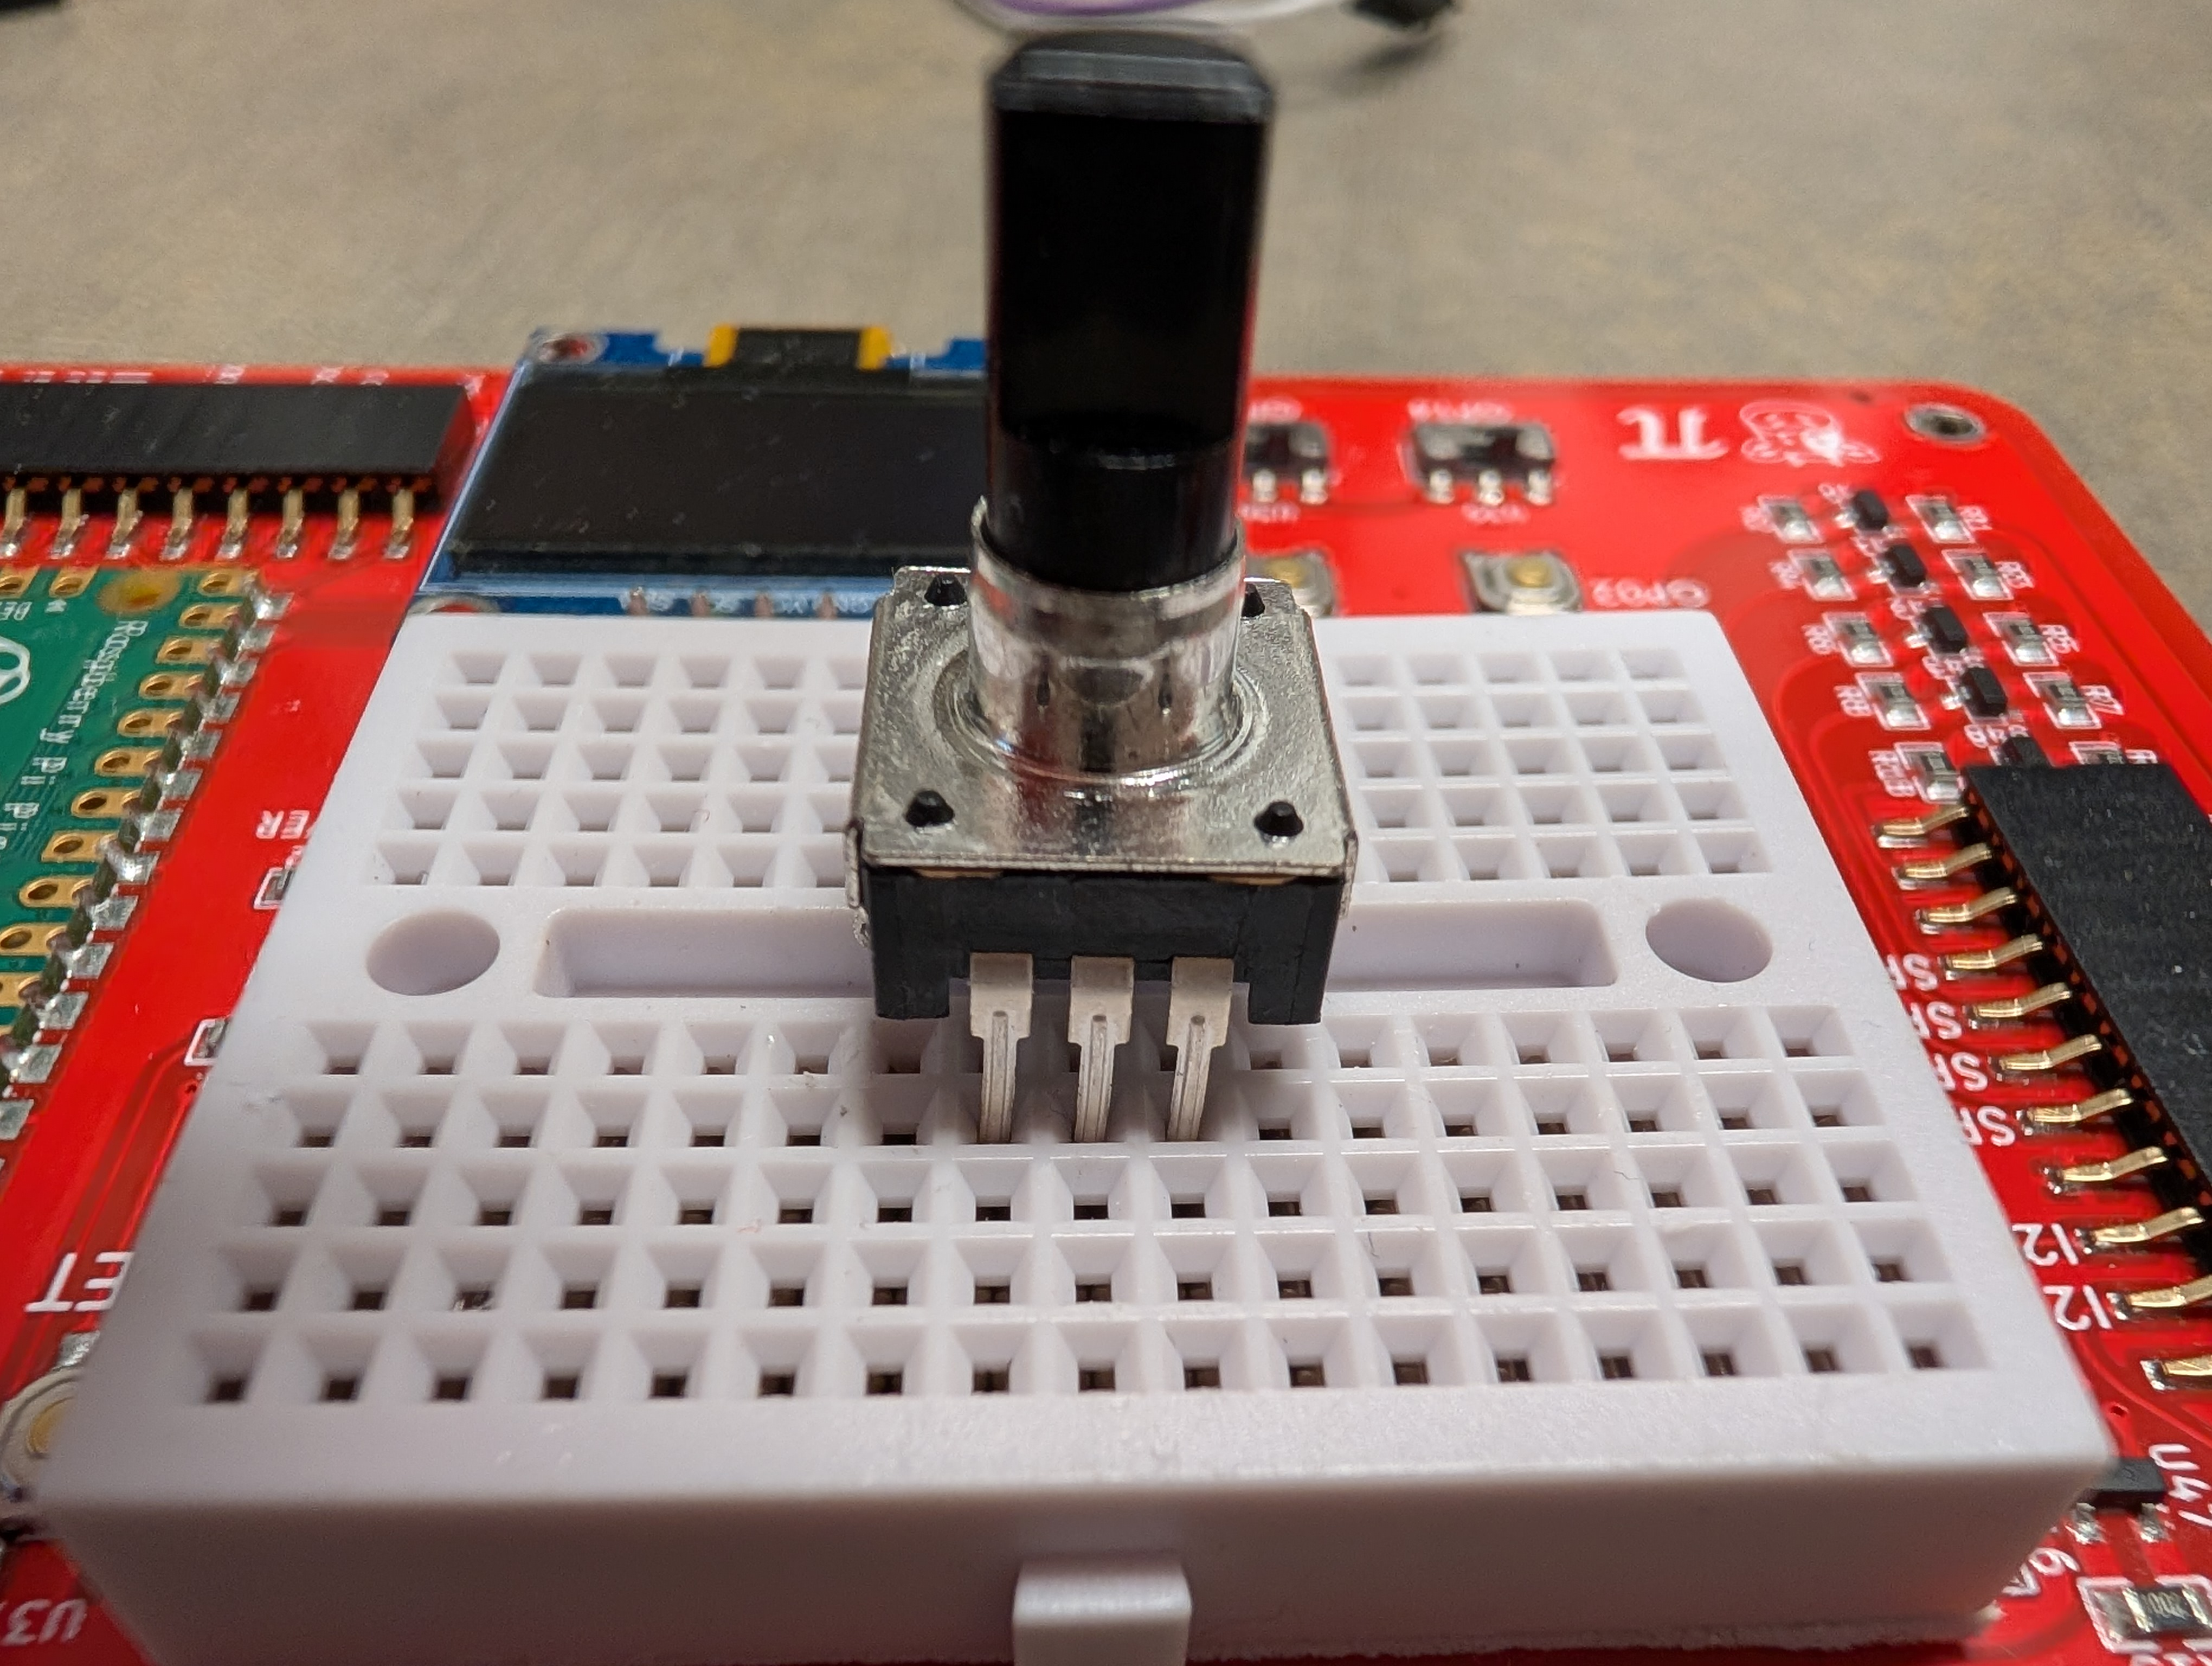
\includegraphics[height=4cm]{hardware/rotaryEncoderPins}
        \label{fig:rotaryEncoderPins}
    }
    \\
    \subfloat[The rotary encoder in the breadboard.]{
        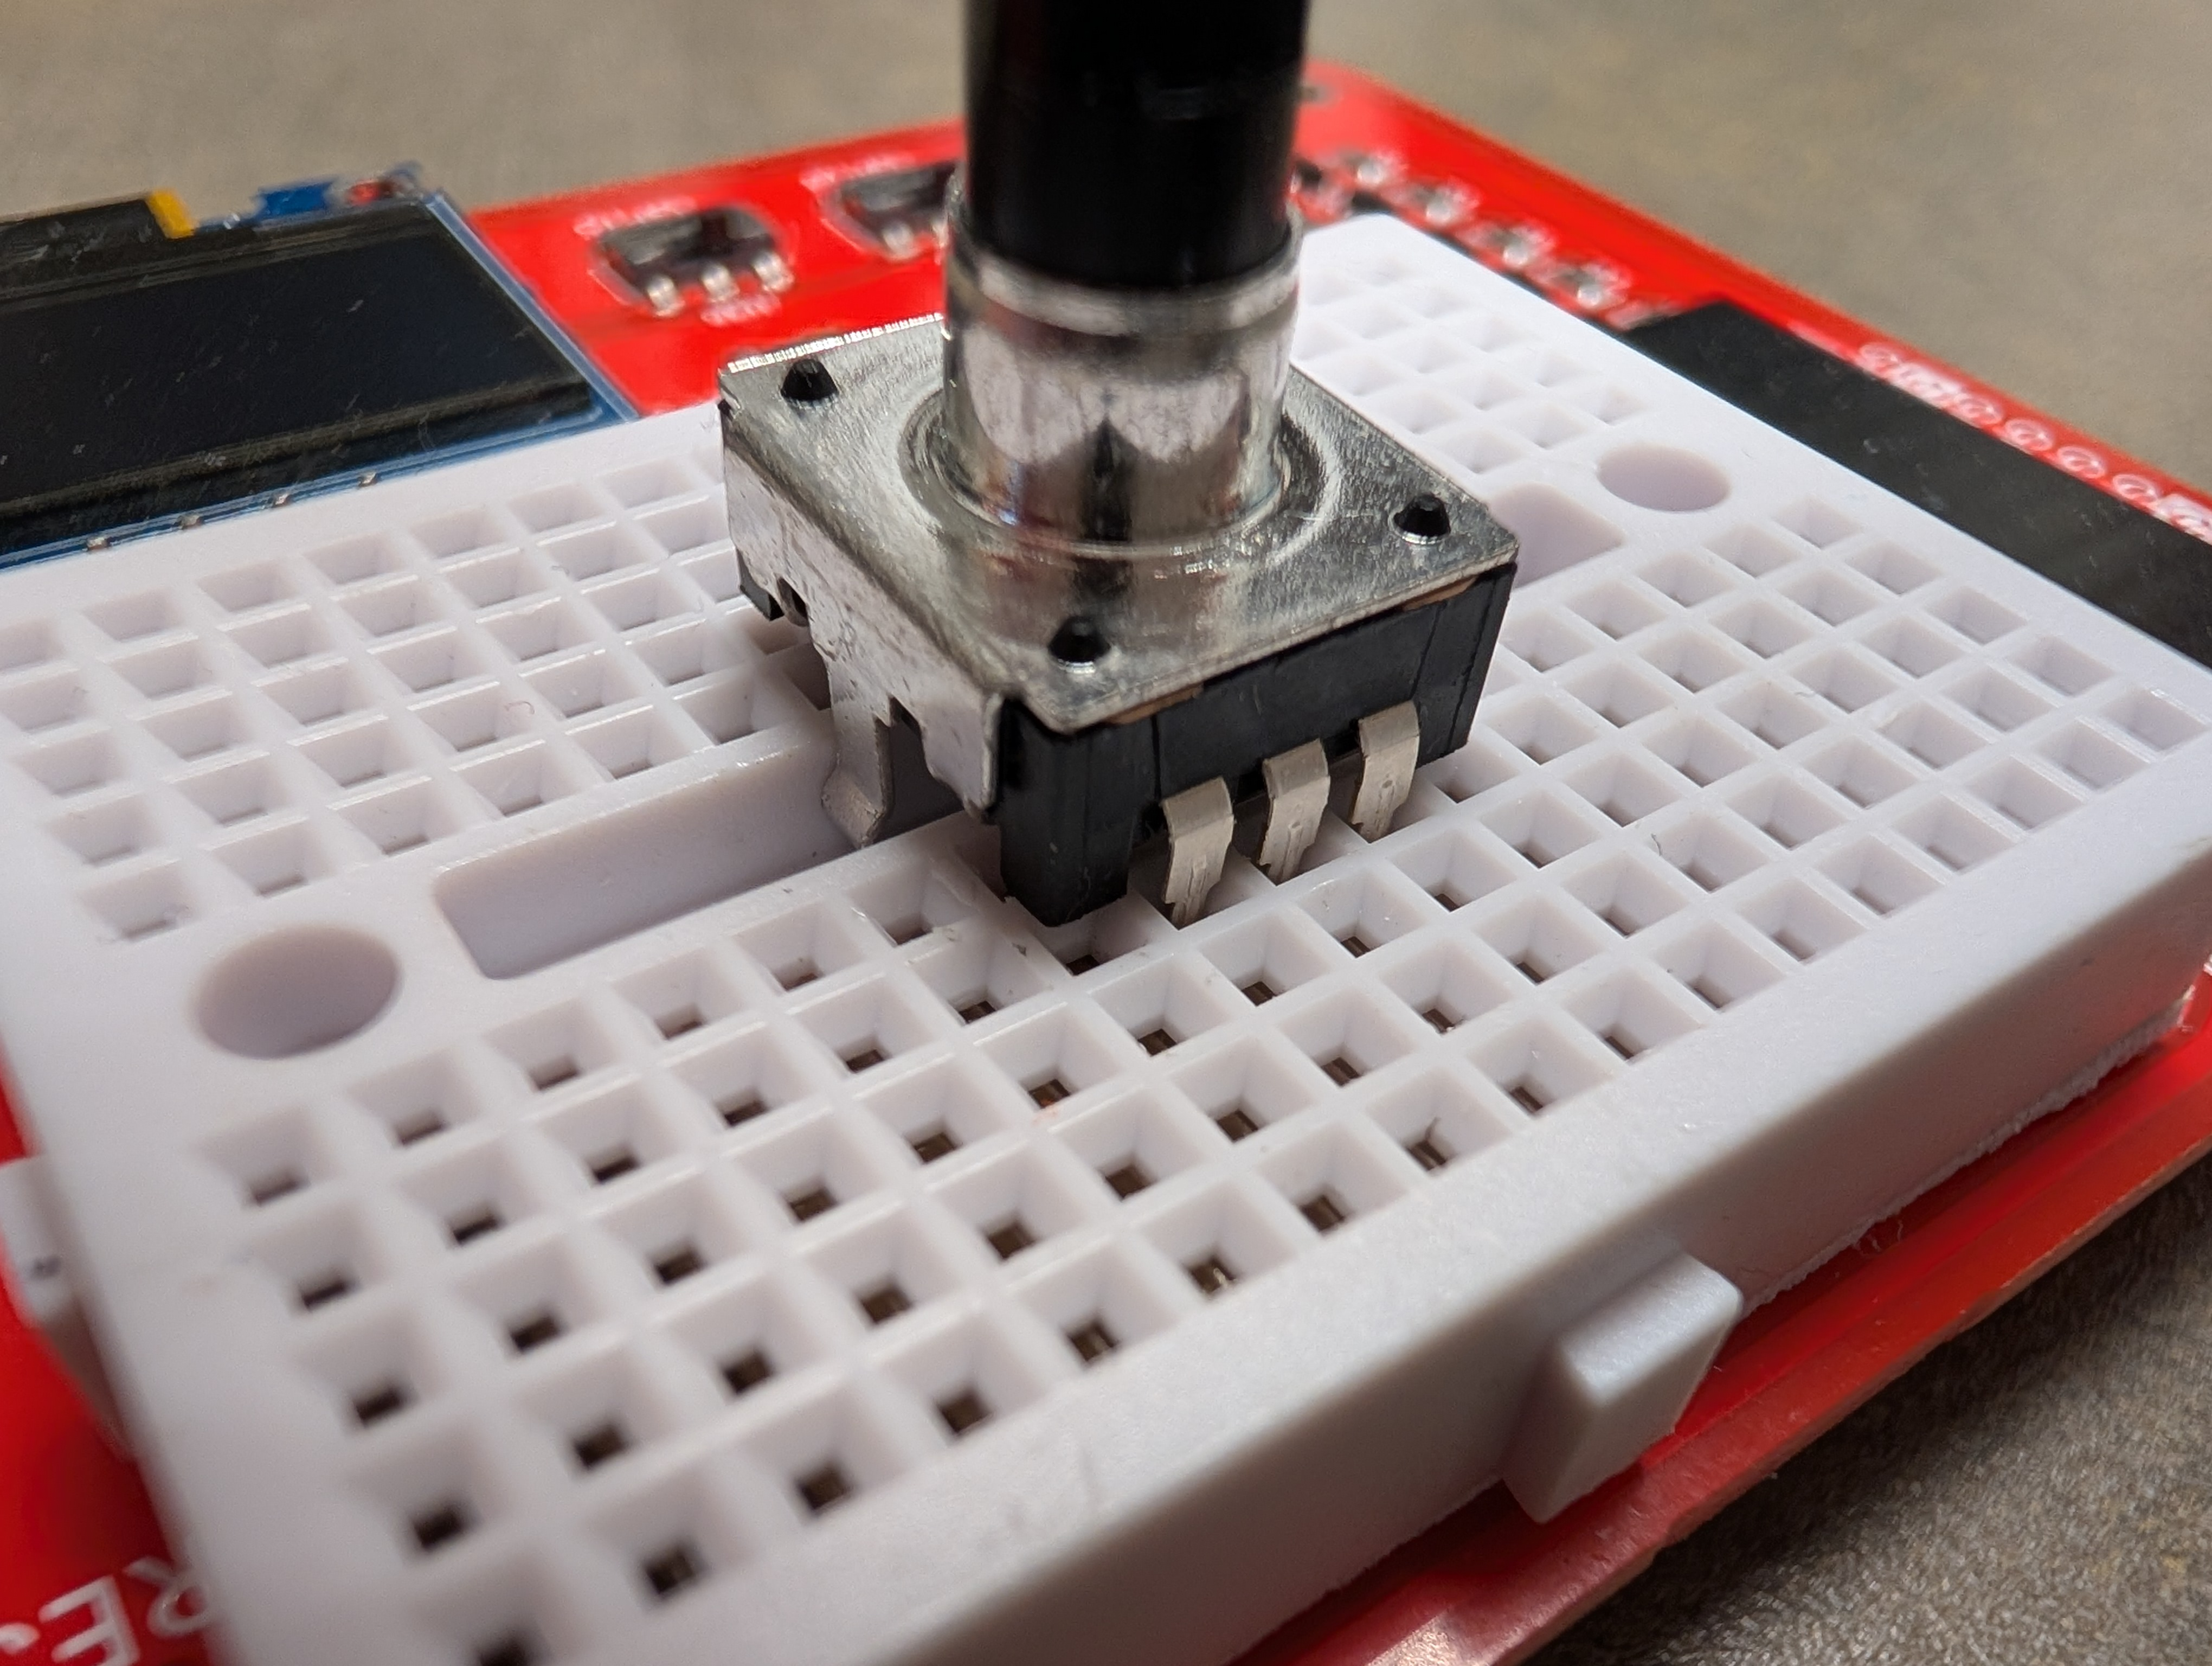
\includegraphics[height=4cm]{hardware/rotaryEncoderInserted}
        \label{fig:rotaryEncoderInserted}
    }
    \\
    \subfloat[Lining up the wires.]{
        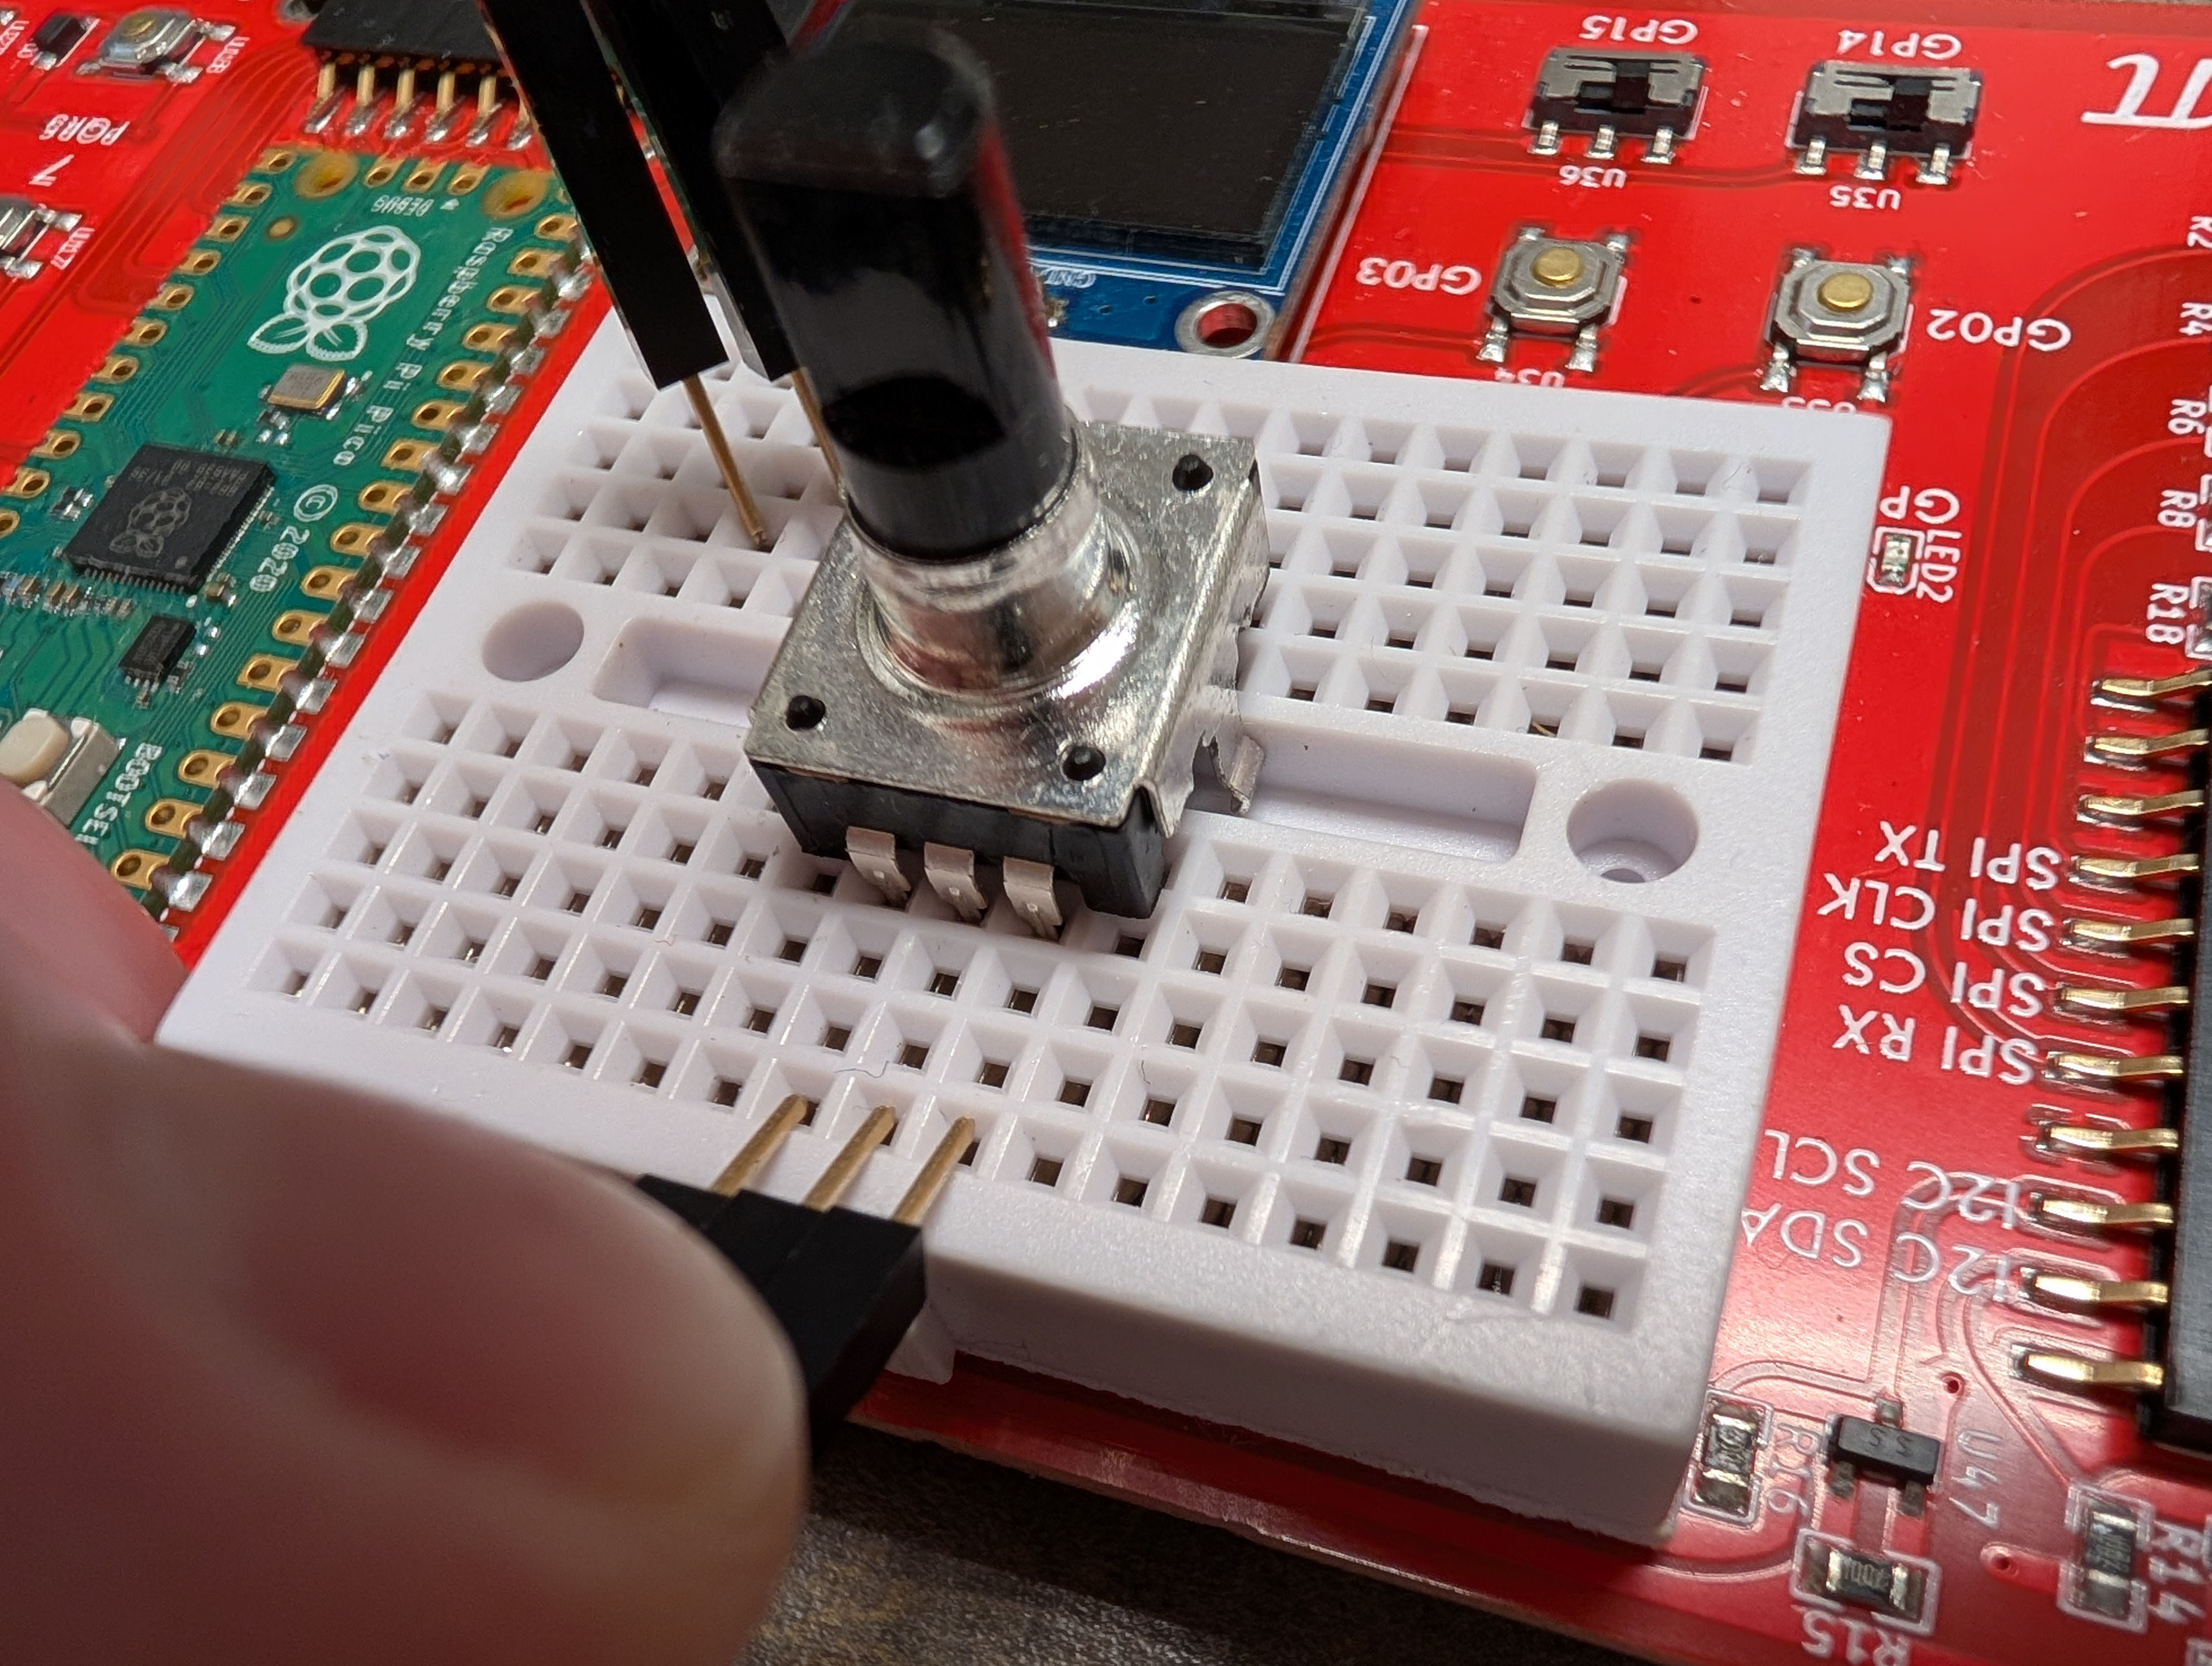
\includegraphics[height=4cm]{hardware/rotaryEncoderAligningWires}
        \label{fig:rotaryEncoderAligningWires}
    }
    \hfil
    \subfloat[Wires connected to the rotary encoder.]{
        \includegraphics[height=4cm]{hardware/rotaryEncoderWiresBreadboard}
        \label{fig:rotaryEncoderWiresBreadboard}
    }
    \caption{Inserting the rotary encoder in the breadboard. \label{fig:rotaryEncoderBreadboard}}
\end{figure}

\begin{description}
    \checkoffitem{Position the rotary encoder on the breadboard so that the prongs on either side of the encoder will fit in the breadboard's gutter (Figure~\ref{fig:rotaryEncoderProngs}),
        and with the three pins positioned in the wells of three contact points (Figure~\ref{fig:rotaryEncoderPins}).}
    \checkoffitem{Gently but firmly, press on the rotary encoder until the bottom of the encoder is flush with the top of the breadboard (Figure~\ref{fig:rotaryEncoderInserted}).}
    \checkoffitem{Insert three 20cm wires, one into each of the same terminal strips that the rotary encoder uses (Figure~\ref{fig:rotaryEncoderAligningWires}--\ref{fig:rotaryEncoderWiresBreadboard}).
        Make a note of which color wire corresponds to which of the sensor's pins.}
\end{description}

The three pins are connected to the rotary encoder's \texttt{A} and \texttt{B} wipers, and to a \texttt{C}ommon ground.
See Figure~\ref{fig:rotaryEncoderLabels} for a labeling of the pins.

\begin{figure}
    \centering
    \subfloat[Labeled pins]{
        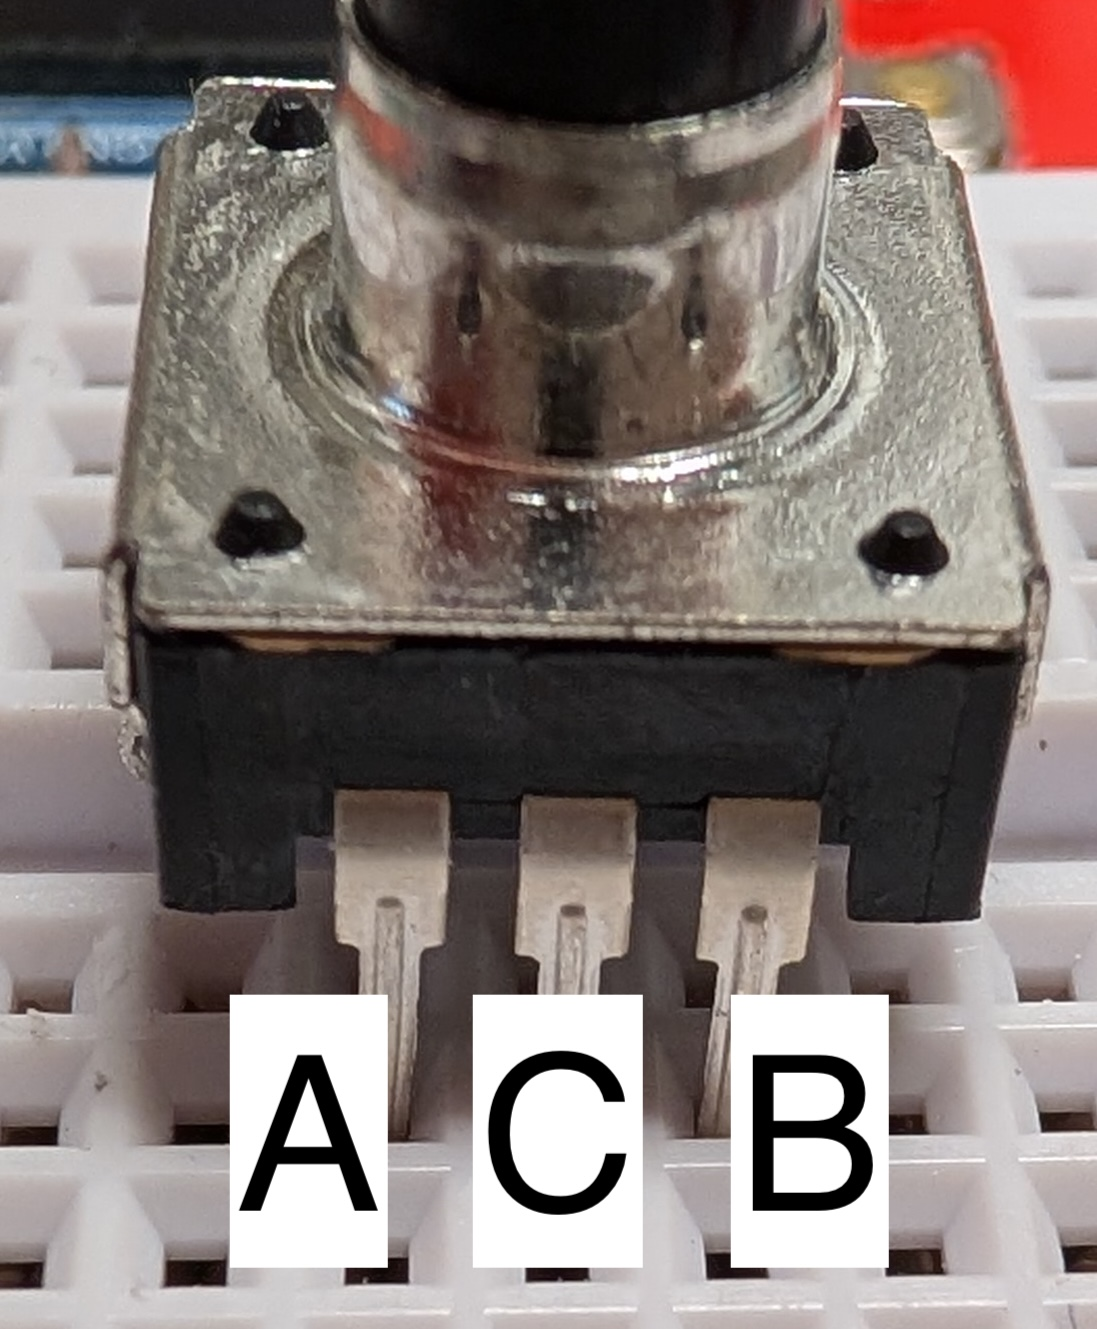
\includegraphics[height=4cm]{hardware/rotaryEncoderPins-labeled}
        \label{fig:rotaryEncoderLabels}
    }
    \hfil
    \subfloat[Inserting the ground wire] {
        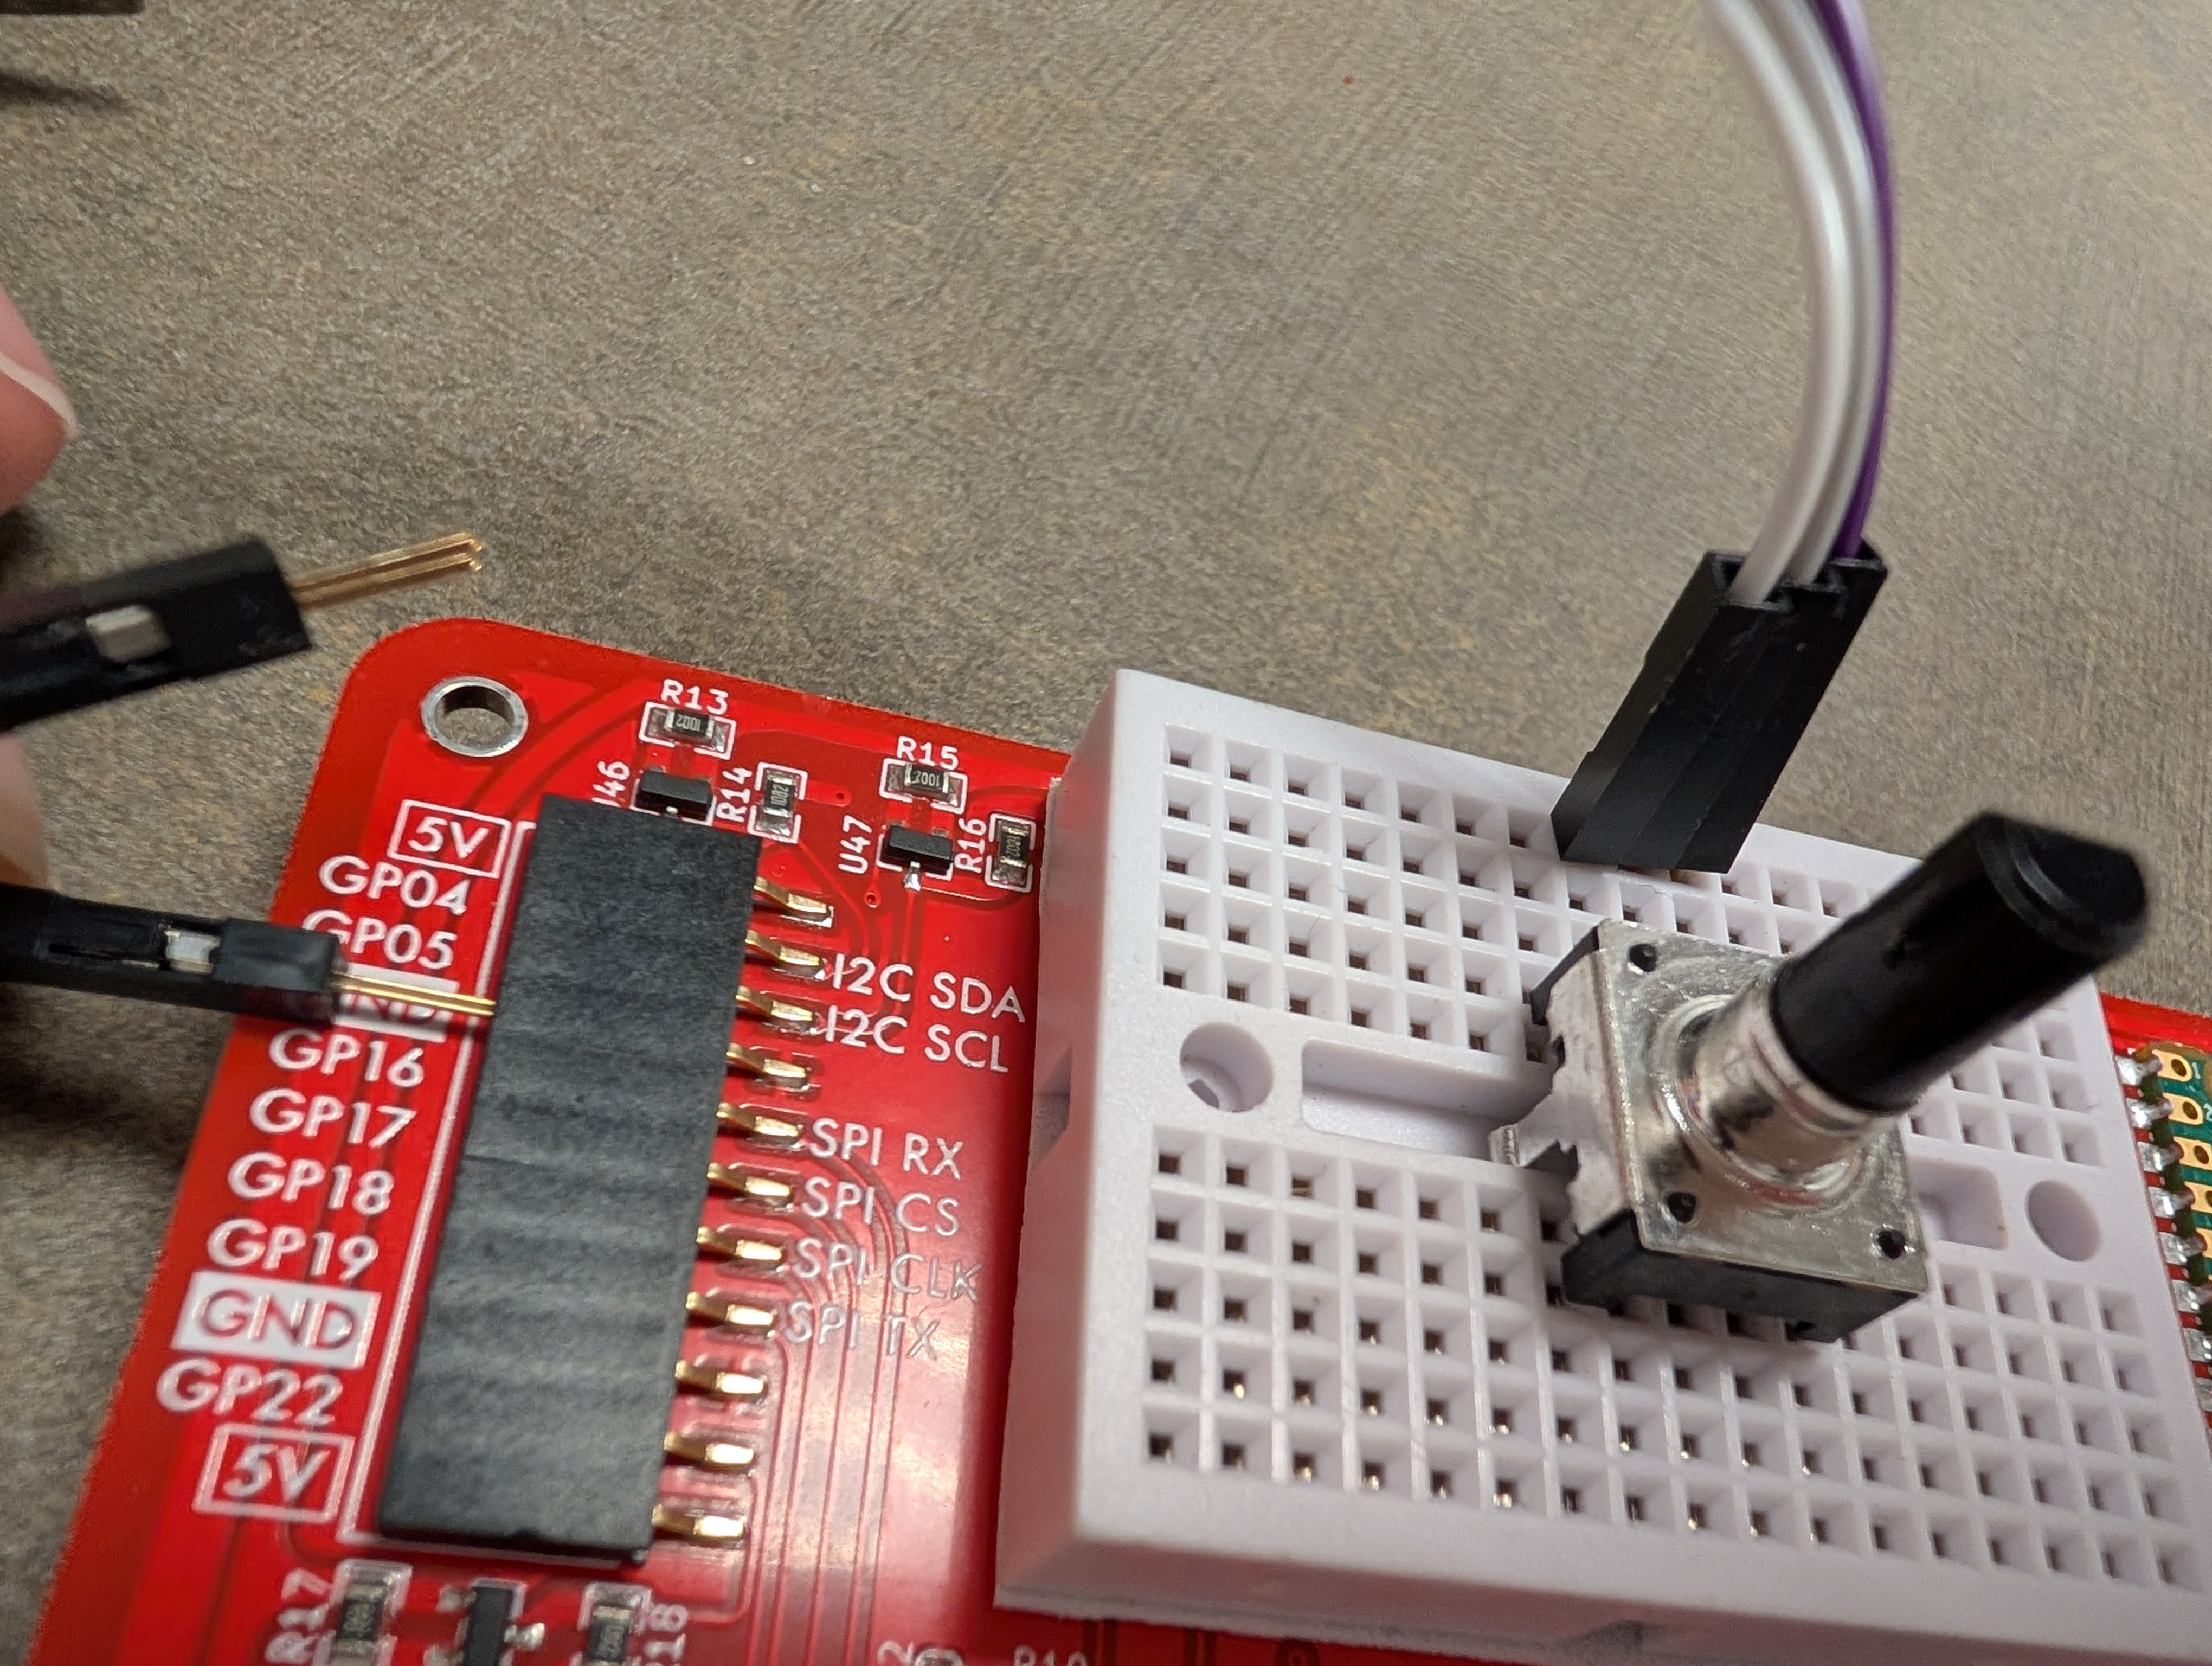
\includegraphics[height=4cm]{hardware/rotaryEncoderGround}
        \label{fig:rotaryEncoderGround}
    }
    \\
    \subfloat[Inserting the A wiper's wire] {
        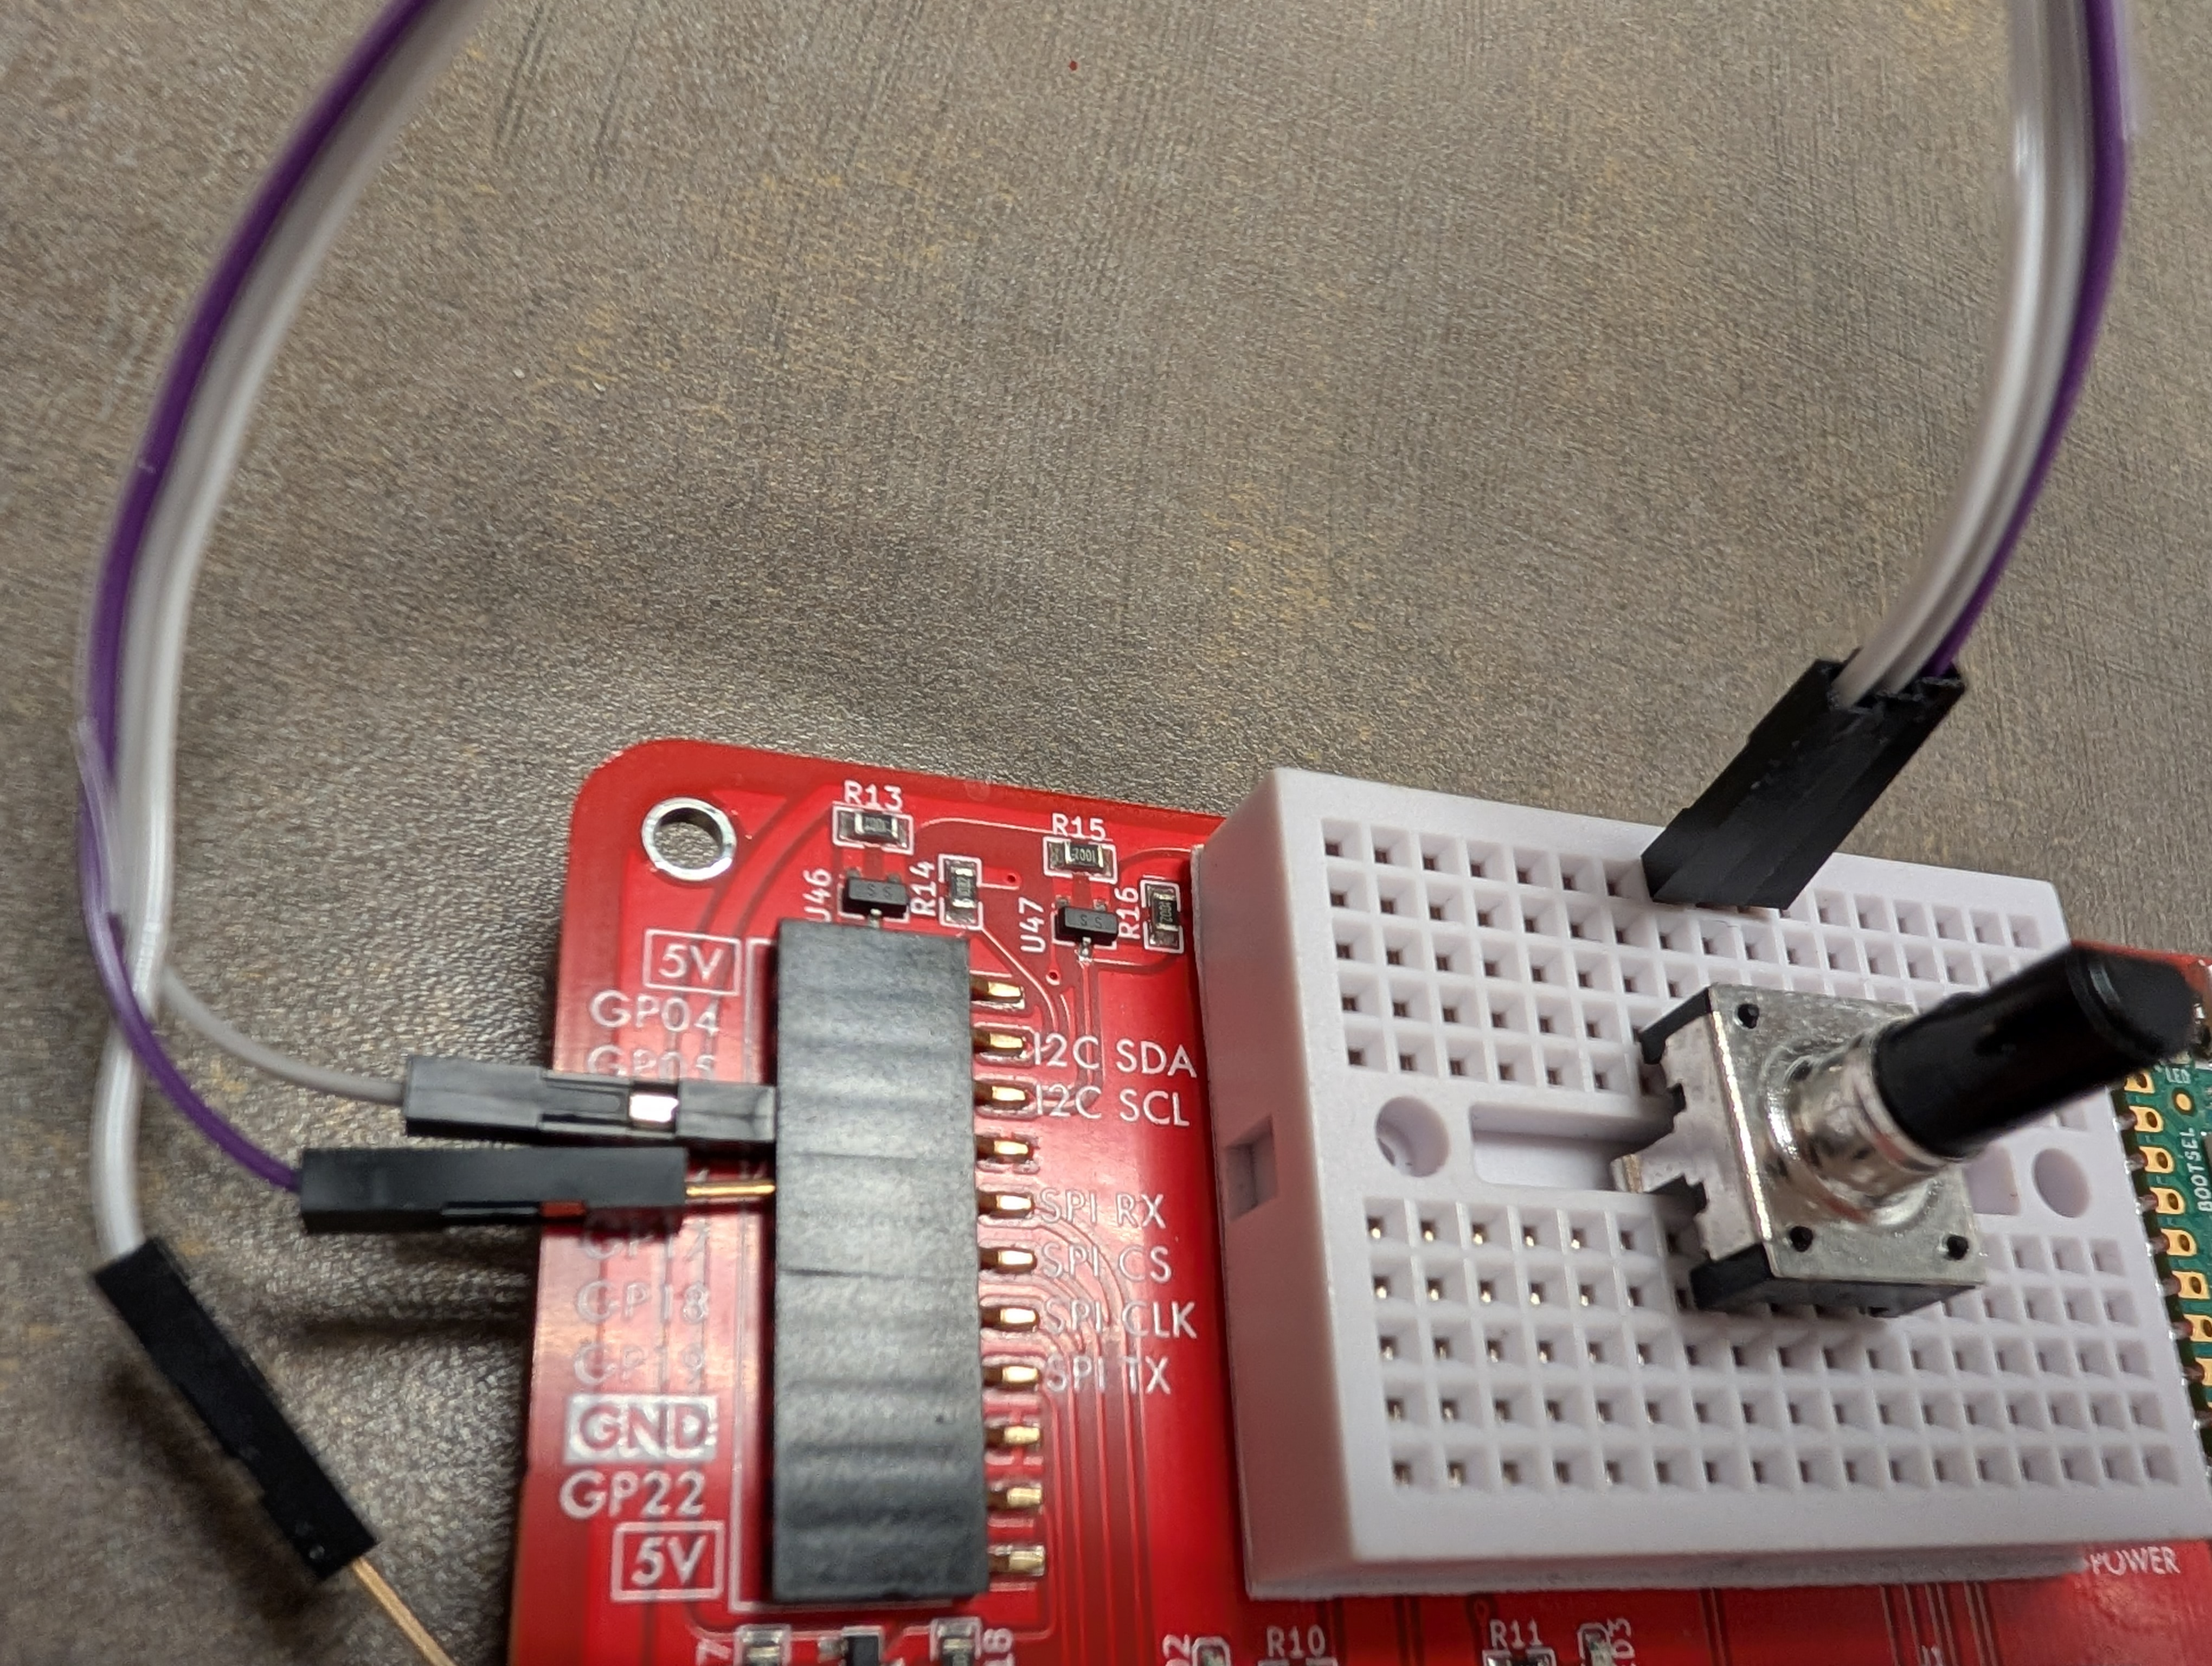
\includegraphics[height=4cm]{hardware/rotaryEncoderApin}
        \label{fig:rotaryEncoderApin}
    }
    \hfil
    \subfloat[Inserting the B wiper's wire] {
        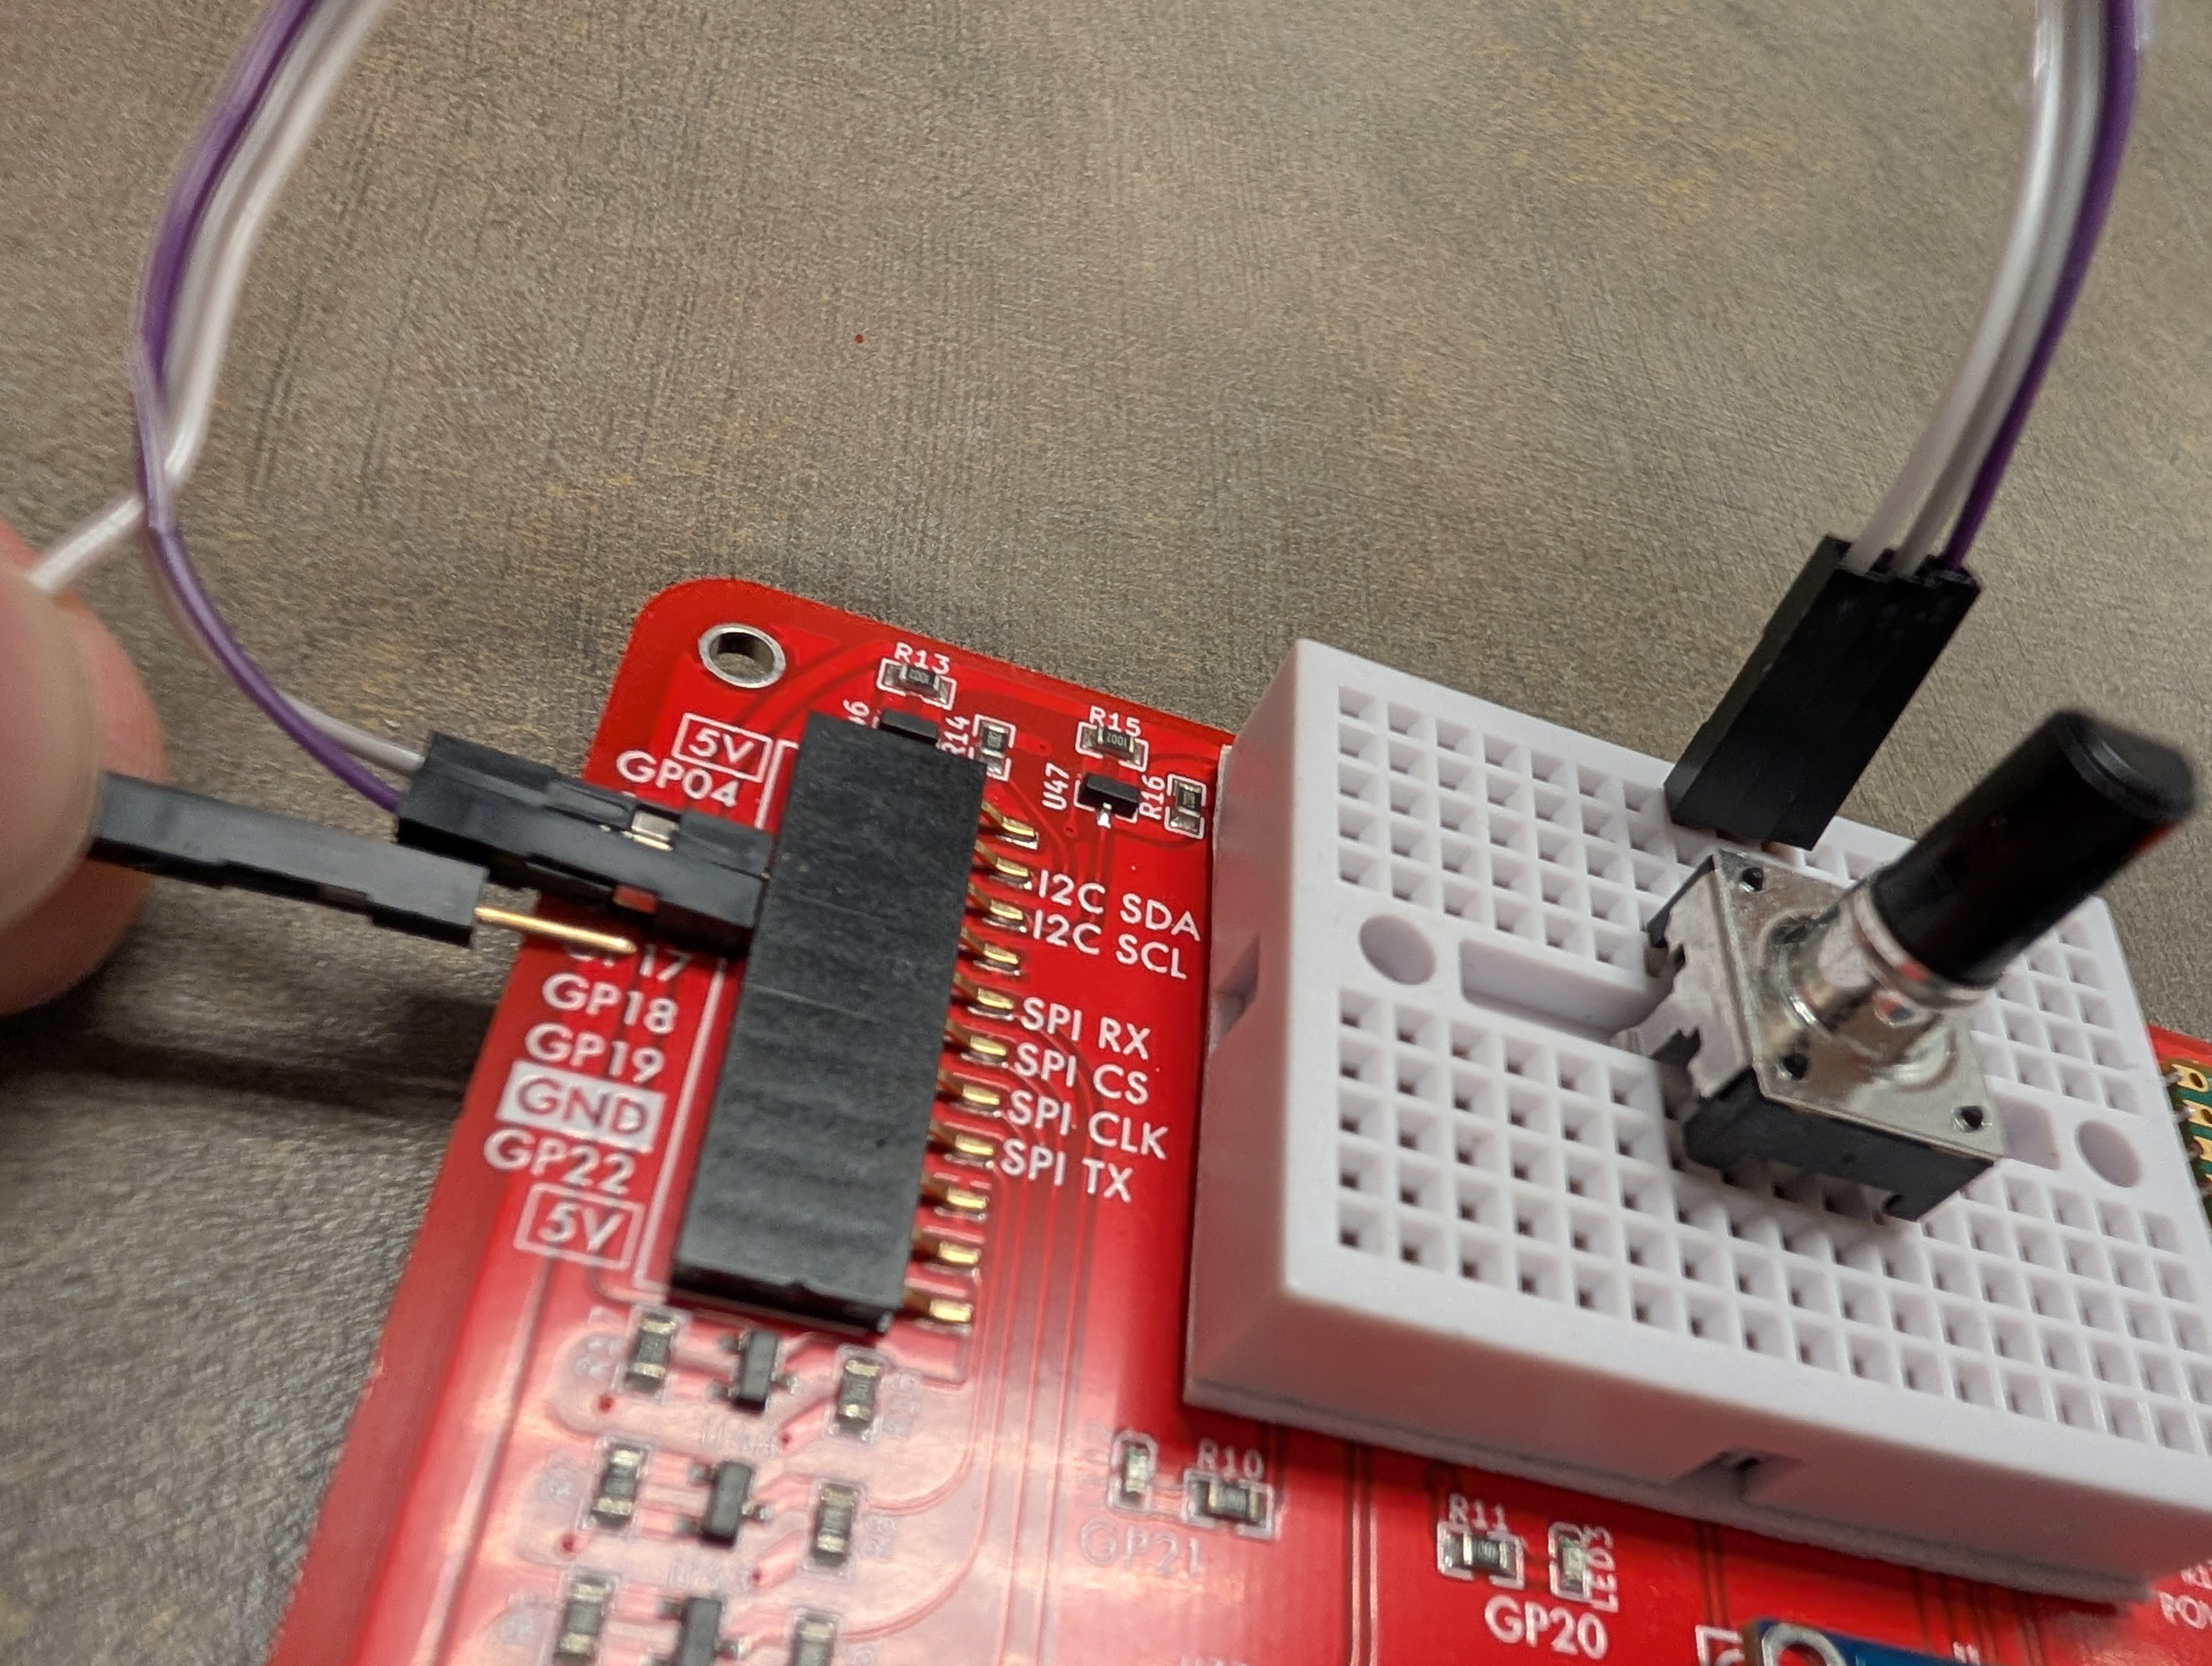
\includegraphics[height=4cm]{hardware/rotaryEncoderBpin}
        \label{fig:rotaryEncoderBpin}
    }
    \caption{Wiring a rotary encoder to the Cow~Pi.}
\end{figure}

\begin{description}
    \checkoffitem{Locate the 20cm that is attached to the rotary encoder's \textbf{\texttt{C}} pin. Insert the other end into a \texttt{GND} slot (Figure~\ref{fig:rotaryEncoderGround}).}
    \checkoffitem{Locate the 20cm that is attached to the rotary encoder's \textbf{\texttt{A}} pin. Insert the other end into the \texttt{GP16} slot.}
    \checkoffitem{Locate the 20cm that is attached to the rotary encoder's \textbf{\texttt{B}} pin. Insert the other end into the \texttt{GP17} slot.}
    \checkoffitem{\textcolor{red}{Have someone verify that you have each wire inserted into the correct slot.}}
\end{description}

The rotary encoder's quadrature can now be read through the Raspberry Pi Pico's pins \texttt{GP16}--\texttt{GP17}.
The starter code will configure \texttt{GP16} \& \texttt{GP17} to be pulled-up input pins.


\vspace{1cm}

Your Cow~Pi is now ready for you to design and code the software for an electronic combination lock.

\begin{figure}[h]
    \centering
    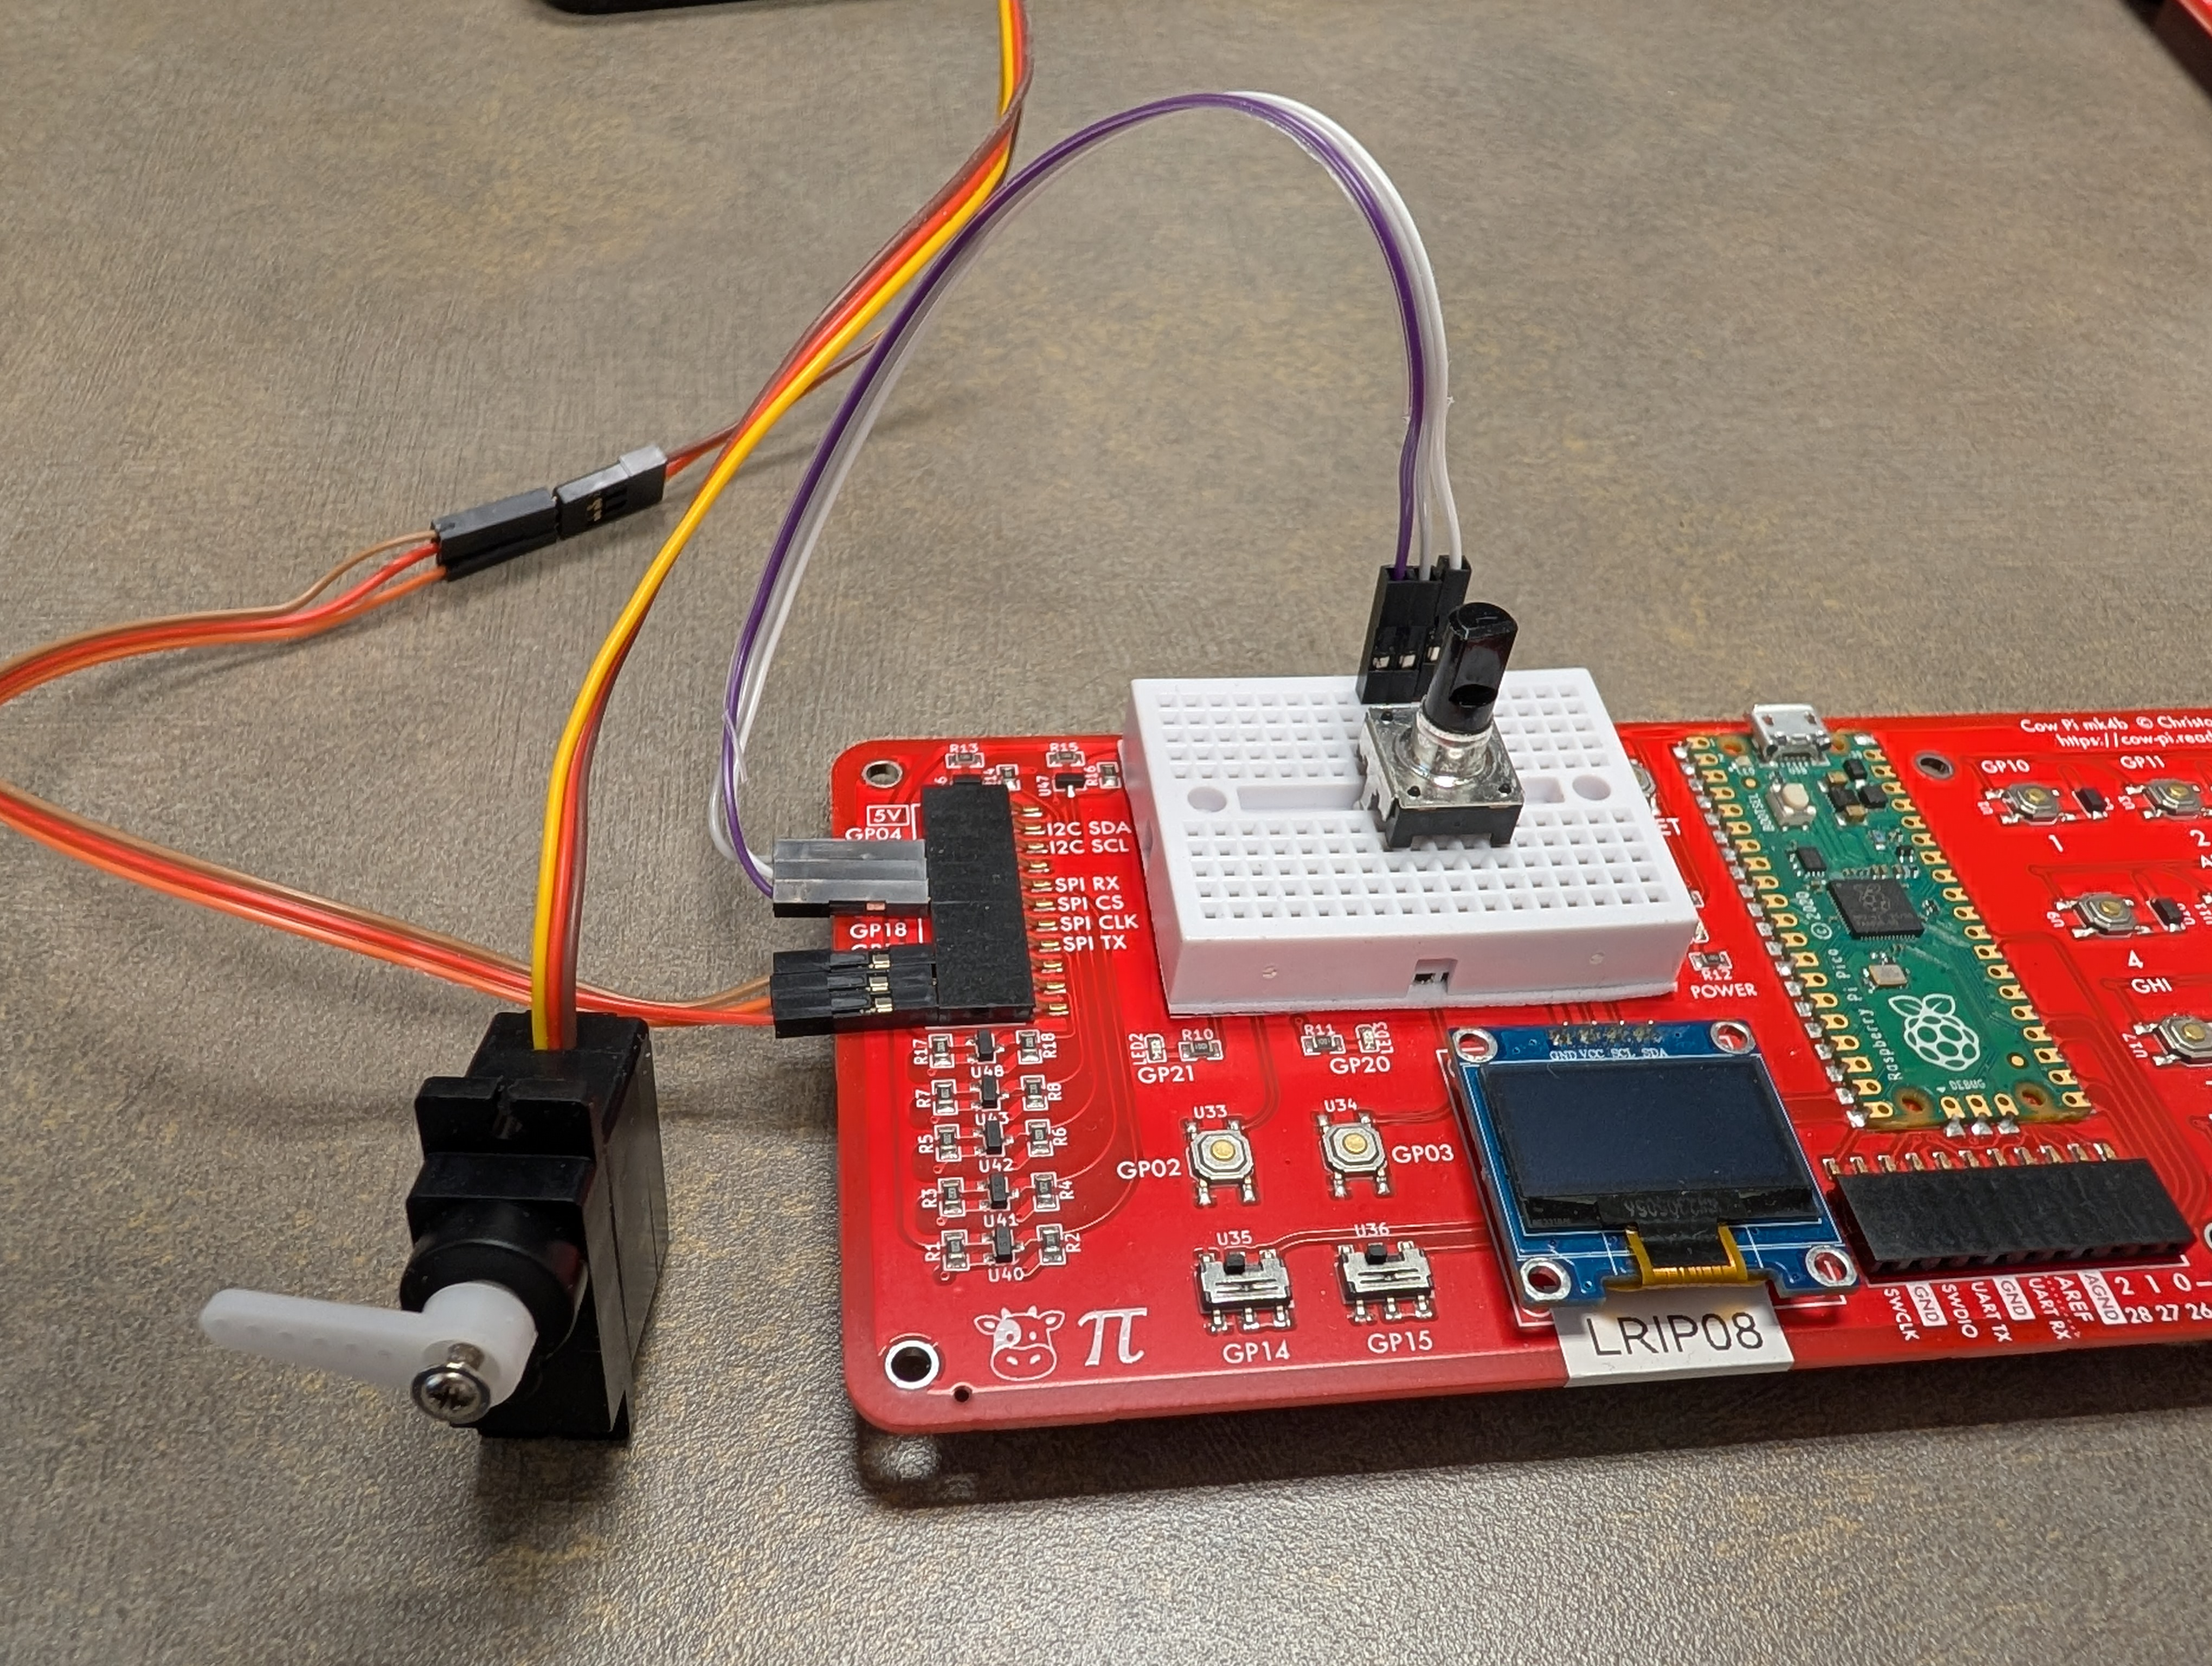
\includegraphics[height=8cm]{hardware/combolock}
    \caption{A fully-assembled combination lock.}
\end{figure}
